\chapter {Analýza a návrh webovej aplikácie}
\todo {popísať kapitolu}

\section {Analýza mriežky ako nástroja}
Cieľom tejto sekcie je zhrnúť požiadavky kladené na štruktúru mriežky, ktorá sa bude vykreslovať nad zobrazenými DICOM snímkami. Obsahom tejto sekcie je aj zhrnutie nastaviteľných parametrov tejto mriežky používateľom.

\subsection {Štruktúra mriežky}
Mriežka pozostáva z horizontálnych a vertikálnych úsečok, ktoré sa navzájom pretínajú. Body, v ktorých sa  úsečky pretínajú, nazveme \uv{hlavnými} bodmi. Tie viažu horizontálnu a vertikálnu úsečku prechádzajúcu týmto bodom. To znamená, že posunutím tohto bodu by malo taktiež dojsť k úprave pozícií úsečiek tak, aby stále prechádzali cez presunutý bod.

Okrem spomenutých bodov by mala aplikácia vykresliť aj takzvané \uv{refinement} body na mriežke, ktoré by sa nachádzali medzi bodmi viažucími úsečky. Ich účel je presnejšie zarovnanie mriežky voči mriežke generovanej technikou SPAMM. V súčasnej aplikácii sa generujú tri \uv{refinement} body medzi každými dvoma \uv{hlavnými} bodmi.

Vykreslená mriežka by mala byť interaktívna, t.j. úprava jej celkovej polohy alebo polohy samotného bodu by malo byť možné pomocou pohybom myši.

\subsection {Nastaviteľné parametre mriežky}\label{grid_settings}
Implementácia mriežky by mala obsahovať nastaviteľné parametre, pomocou ktorých by sa dala meniť jej vzhľad, resp. štruktúra.

Zoznam všetkých parametrov mriežky, ktoré by mali byť upraviteľné používateľom, je nasledovný:
\begin {itemize}
\item {uhol mriežky,}
\item {priestor medzi všetkými bodmi,}
\item {X a Y offset mriežky počítaný z ľavého horného rohu snímky a}
\item {počet horizontálnych a vertikálnych úsečiek.}
\end {itemize}

Horeuvedené parametre by mali byť upraviteľné pomocou vstupu na klávesnici.
Taktiež bude môcť byť upraviteľná poloha samotnej mriežky alebo jej akéhokoľvek bodu pomocou myši. Okrem toho by malo byť možné implementovať prepínač, ktorý zaistí zobrazenie \uv{refinement} bodov na vykreslenej mriežke a naopak.

Mriežka by mala na úpravy týchto parametrov reagovať jej prekreslením berúcim do úvahy zmenu daného parametru.

\section {Analýza požiadaviek}
Táto sekcia sa venuje analýze požiadaviek, ktoré sa delia na dve hlavné kategórie -- funkčné a nefunkčné požiadavky. Ich realizácia je nutnosťou pre vytvorenie webovej aplikácie, ktorá bude obsahovať potrebnú funkcionalitu pre základ analýzy srdcového myokardu.

\subsection {Funkčné požiadavky}
Funkčné požiadavky sú požiadavky vymedzujúce rozsah funkcionality, ktorá by mala byť v danej aplikácii implementovaná.

\subsubsection {FR1 -- Spracovanie a zobrazenie MR snímiek}\label{fr1}
Do aplikácie by malo byť možné importovať snímky z magnetickej rezonancie vo formáte DICOM a tieto snímky taktiež zobraziť.

\subsubsection {FR2 -- Animácia MR snímiek}\label{fr2}
Aplikácia by mala umožniť animovať importované snímky pre jednoduchšiu analýzu pohybu myokardu. Parametre animácie ako jej rýchlosť a výber snímky, od/po ktorej/ktorú má animácia prebiehať, by mali byť upraviteľné, napr. pomocou číselného vstupu.

\subsubsection {FR3 -- Zobrazenie a interaktívna úprava mriežky}\label{fr3}
Implementovaná aplikácia by mala vedieť zobraziť mriežku nad snímkou z MR, ktorá by sa mala dať vygenerovať tlačidlom v používateľskom rozhraní. Taktiež je nutné implementovať nastaviteľné parametre mriežky, ktoré boli popísané v sekcii \ref{grid_settings}. Zmena týchto parametrov by mala byť ihneď viditeľná používateľom.

\subsubsection {FR4 -- Zadanie parametrov pre SPAMM algoritmus}\label{fr4}
Pre korektný výpočet súradníc bodov mriežok je nutné funkčnému SPAMM algoritmu podsunúť rozličné parametre. Ich hodnoty by sa mali dať určiť v aplikácií pre ich neskoršie použitie v tomto algoritme. Výpis týchto parametrov je možné nájsť v \ref{helper_apps}.

\subsubsection {FR5 -- Spustenie SPAMM algoritmu a zobrazenie jeho výsledkov}\label{fr5}
SPAMM algoritmus prijme potrebné dáta o všetkých importovaných snímkach a na nich definovaných mriežkach. Výstupom tohto algoritmu bude štruktúra dát, ktorá bude zodpovedať mriežkam s popisom súradníc bodov. Tento výstup bude následne nutné zobraziť v aplikácii.

\subsection {Nefunkčné požiadavky}
Požiadavky tohto typu síce nevymedzujú rozsah funkcionality danej aplikácie, avšak umožňujú určiť isté obmedzenia pre novú aplikáciu, ako napr. dôraz na podobu výslednej architektúry tejto aplikácie.

\subsubsection {NF1 -- Webová aplikácia}
Prvou nefunkčnou požiadavkou je vytvorenie webovej aplikácie, ktorá by mala byť prístupná zo všetkých moderných webových prehliadačov. Pre lekárov výber tejto architektúry zjednoduší jej prístupnosť, nakoľko k takejto aplikácii bude možné pristupovať z rôznych zariadení a platforiem bez nutnosti inštalácie aplikácie.

\subsubsection {NF2 -- Používateľské rozhranie}
Pre interakciu s aplikáciou je nutné navrhnúť a implementovať používateľské rozhranie, pomocou ktorého bude možné s aplikáciou interagovať. Lekári by preferovali používateľské rozhranie podobné iným aplikáciám z tejto oblasti.

\subsubsection {NF3 -- Ochrana pred únikom dát o pacientovi}
Práca s osobnými dátami by mala byť do maximálnej možnej miere naprieč aplikáciou minimalizovaná, aby sa predišlo únikom citlivých údajov o pacientovi. Týka sa to najmä práce s DICOM súbormi, nakoľko tie obsahujú citlivé dáta o pacientovi.

\section {Používateľské role}
V aplikácii sa bude nachádzať len jeden aktér -- používateľ, rovnako ako v súčasnej aplikácii. Tomuto aktérovi by mala byť aplikácia sprístupnená bez rôznych funkčných obmedzení.

\section {Prípady použitia}
Nasledujúce prípady použitia reprezentujú rôzne činnosti, ktoré môže používateľ s aplikáciou vykonávať. Tieto prípady použitia sú popísané pomocou scenárov, ktoré vychádzajú z funkčných požiadaviek kladených na novú aplikáciu.

Pre lepšiu predstavu sú prípady použitia taktiež znázornené graficky pomocou Use Case diagramu na nasledujúcej strane.

\begin {figure}[H]
        \centering
        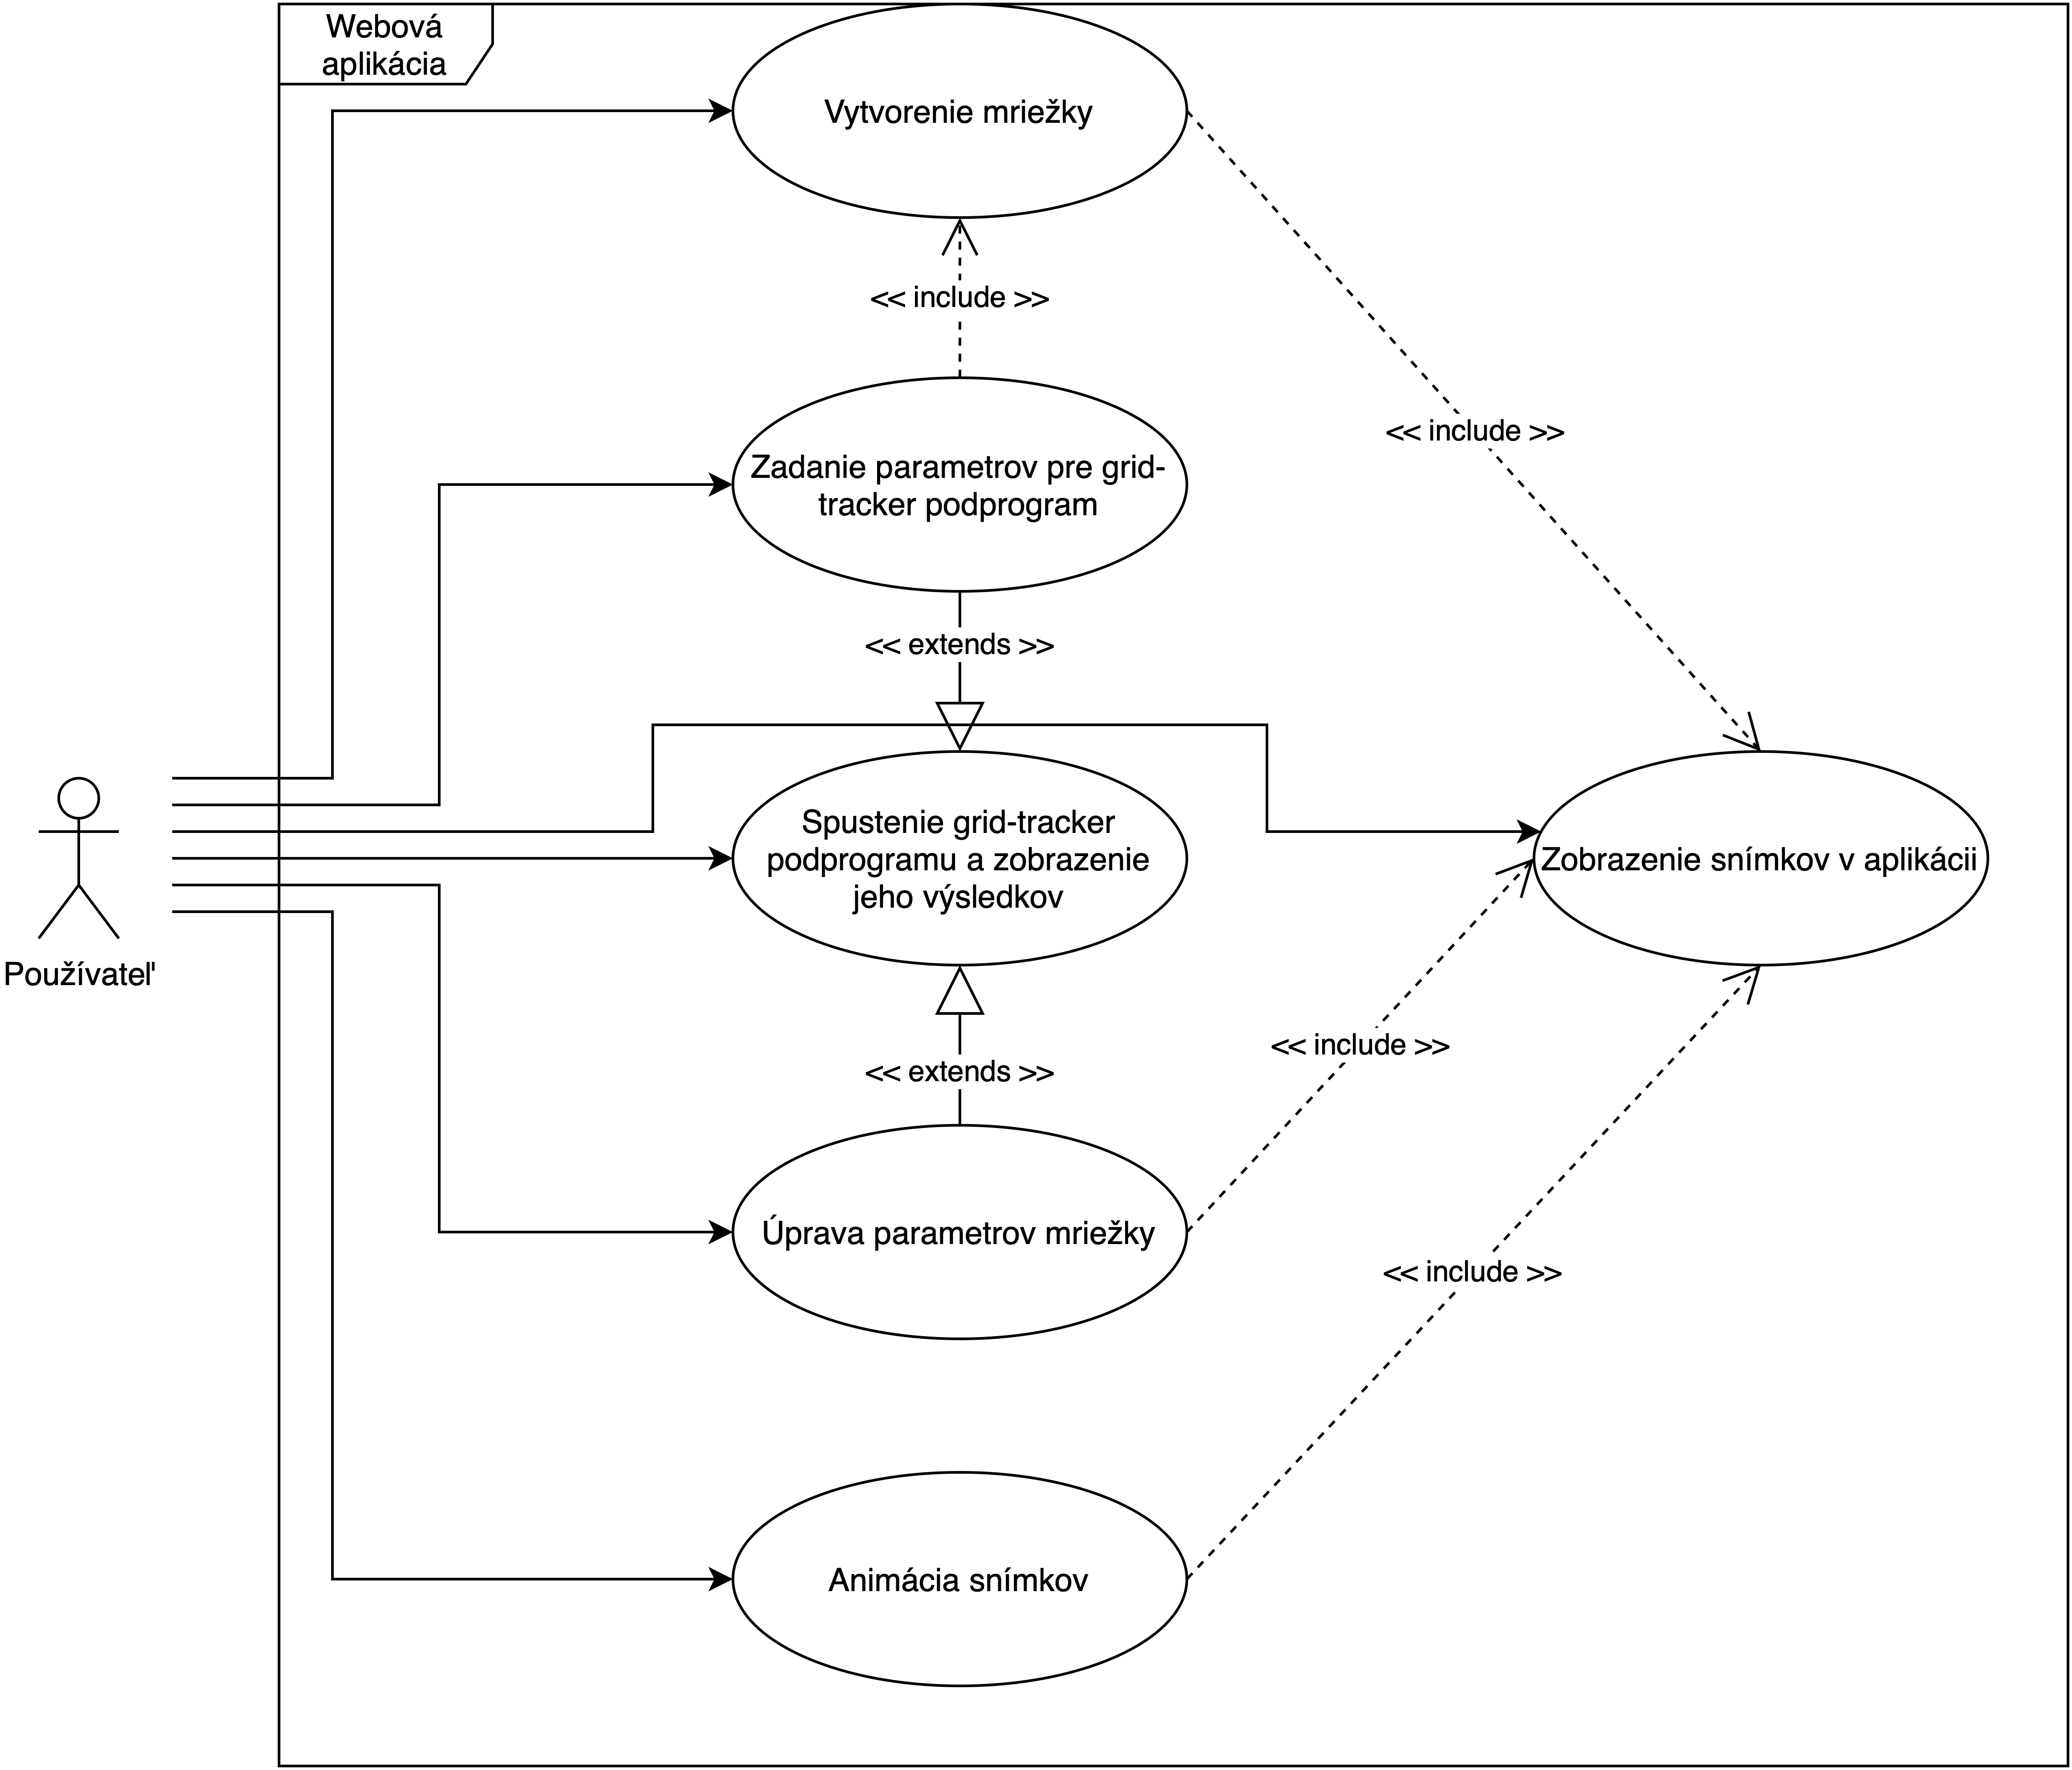
\includegraphics[height=10cm]{media/graphs/usecase.png}
        \captionsetup{justification=centering}
        \captionof{figure}[Use case diagram]{Use case diagram}
\end {figure}

\subsection {UC1 -- Zobrazenie snímiek v aplikácii}\label{uc1}
Zobrazenie snímiek magnetickej rezonancie v DICOM formáte je jedným z esenciálnych funkčných požiadaviek -- \uv{\nameref{fr1}}. Nasledovný scenár túto požiadavku realizuje.

\subsubsection*{Scenár:}
\begin {enumerate}
\item {Používateľ klikne na jedno z tlačidiel pre import DICOM snímiek do aplikácie.}
\item {Prehliadač zobrazí systémové okno, v ktorom si používateľ vyberie snímky, ktoré by chcel mať zobrazené v aplikácii.}
\item {Následne potvrdí import želaných snímiek.}
\item {Aplikácia automaticky vykreslí prvú importovanú snímku a taktiež zobrazí náhľady ostatných importovaných snímiek.}
\item {V prípade, že sa medzi zvolenými snímkami nachádza súbor, ktorý nekorešponduje so štruktúrou DICOM súboru, aplikácia zobrazí notifikáciu o neúspešnom zobrazení snímky.}
\end {enumerate}
	
\subsection {UC2 -- Animácia snímiek}\label{uc2}
Nasledovný scenár realizuje funkciu prehrania série snímiek ako animáciu, ako bolo popísané vo funkčnej požiadavke \uv{\nameref{fr2}}.
Okrem iného taktiež zahŕňa prípad \uv{\nameref{uc1}}. 

\subsubsection*{Scenár:}
\begin {enumerate}
\item {\nameref{uc1}.}
\item {Kliknutím na tlačidlo reprezentujúce štart animácie sa spustí animácia importovaných snímiek.}
\item {Kliknutím na tlačidlo reprezentujúce koniec animácie sa animácia skončí.}
\end {enumerate}

\subsubsection*{Alternatívny scenár:}
\begin {enumerate}
\item [\textbf{2.}] {Používateľ si nastaví rýchlosť animácie, index snímky, od ktorej má animácia začínať alebo index snímky, ktorou má animácia končiť.}
\item  [\textbf{3.}] {Kliknutím na tlačidlo reprezentujúce štart animácie sa spustí animácia importovaných snímiek.}
\item  [\textbf{4.}] {Kliknutím na tlačidlo reprezentujúce koniec animácie sa animácia skončí.}
\end {enumerate}

\subsection {UC3 -- Vytvorenie mriežky}\label{uc3}
Vytvorenie mriežky nad snímkou z MR je potrebné pre účely analýzu pohybu myokardu. Nasledujúci scenár čiastočne realizuje funkčnú požiadavku -- \uv{\nameref{fr3}}. Taktiež zahŕňa prípad použitia \uv{\nameref{uc1}}.

\clearpage

\subsubsection*{Scenár:}
\begin {enumerate}
\item {\nameref{uc1}.}
\item {Používateľ klikne na tlačidlo \uv{Create grid}.}
\item {Aplikácia zobrazí výzvu pre kliknutie na oblasť snímky, kde má byť mriežka vytvorená.}
\item {Používateľ klikne na oblasť snímky, kde chce vytvoriť mriežku.}
\item {Aplikácia vygeneruje mriežku s predvolenými nastaveniami a zobrazí ju na mieste predchádzajúceho kliknutia myši.}
\end {enumerate}

\subsection {UC4 -- Úprava parametrov mriežky}\label{uc4}
Medzi prípady použitia patrí aj úprava parametrov mriežky určenej pre analýzu pohybu srdcového svalu. Nakoľko je najprv potrebné mať mriežku pred jej úpravou vytvorenú, zahŕňa nasledovný scenár aj jej vytvorenie. Ten taktiež čiastočne realizuje funkčnú požiadavku \uv{\nameref{fr3}}.

\subsubsection*{Scenár:}
\begin {enumerate}
\item {\nameref{uc3}.}
\item {Používateľ upraví jeden alebo viacero parametrov uvedených v \ref{grid_settings}.}
\item {Aplikácia následne automaticky vykreslí mriežku na základe upravených parametrov.}
\end {enumerate}

\subsection {UC5 -- Zadanie parametrov pre SPAMM algoritmus}\label{uc5}
Pre spustenie algoritmu zodpovedného pre posun mriežky vytvorenej používateľom voči mriežke vygenerovanej SPAMM technikou je potrebné tomuto algoritmu poslať tri parametre definované v \ref{image_processing_tab}. Tieto parametre budú využité pri použití funkčného SPAMM algoritmu. Nasledujúci scenár tento prípad použitia realizuje spolu s funkčnou požiadavkou -- \uv{\nameref{fr4}}.

\clearpage

\subsubsection*{Scenár:}
\begin {enumerate}
\item {\nameref{uc1}.}
\item {Používateľ zadá číselné hodnoty parametrov \uv{Curvature coefficient}, \newline \uv{Force coefficient} a \uv{Stop time}.}
\end {enumerate}

\subsection {UC6 -- Spustenie SPAMM algoritmu a zobrazenie jeho výsledkov}\label{uc6}
Spustenie algoritmu a zobrazenie jeho výsledku vyžaduje mať importované DICOM snímky spolu s používateľom vytvorenými mriežkami a ich modifikáciami.

To je dôvodom, prečo tento scenár použitia zahŕňa prípady \uv{\nameref{uc1}}, \uv{\nameref{uc3}}, \uv{\nameref{uc4}} a \uv{\nameref{uc5}}. Samotný scenár realizuje funkčnú požiadavku \uv{\nameref{fr5}}.

\subsubsection*{Scenár:}
\begin {enumerate}
\item {\nameref{uc1}}.
\item {\nameref{uc3}}.
\item {\nameref{uc4}}.
\item {\nameref{uc5}}.
\item {Používateľ kliknutím na tlačidlo \uv{Compute} spustí výpočet SPAMM algoritmu.}
\item {Po dokončení výpočtu aplikácia zobrazí mriežky upravené horeuvedeným algoritmom.}
\end {enumerate}

\clearpage

\section {Technológie pre vývoj webovej aplikácie}
V rámci tejto analýzy budú popísané technológie, ktoré budú použité pri vývoji webovej aplikácie. Konkrétne balíčky, príp. závislosti sa v tejto sekcii nachádzať nebudú -- tie budú popísané v kapitole implementácie webovej aplikácie.

\subsection {HTML5}
Pre definovanie štruktúry webového dokumentu a jeho významu bude potrebné použiť značkovací jazyk HTML. Tento jazyk pozostáva zo série značiek (elementov) a k nim príslušných atribútov, pomocou ktorých je možné vytvorený obsah anotovať a významovo ho definovať. Týmto spôsobom je možné vytvoriť nadpisy, odstavce textu, číselné i nečíselné zoznamy, či importovať obrázky alebo sprostredkovať audio/video, atď.

Takto štruktúrovaný dokument definovaný pomocou jazyka HTML je možné zobraziť v ľubovoľnom webovom prehliadači. Webový prehliadač takýto dokument zanalyzuje a na základe použitých značiek vykreslí. Každá značka má definovaný predvolený štýl zobrazenia, ktorý sa môže líšiť od prehliadača k prehliadaču.

Nižšie je uvedený príklad základnej štruktúry HTML5 webového dokumentu:

\begin{minipage}[]{\linewidth}
\begin{minted}{html}
<!doctype html5>
<html>
  <head></head>
  <body>
    <p>Hello world!</p>
  </body>
</html>
\end{minted}
\end{minipage}

Značka \texttt{<!doctype>} definuje verziu použitého HTML dokumentu, čo je v tomto prípade HTML5. Ďalej nasleduje značka \texttt{<html>}, ktorej úloha je zoskupiť elementy \texttt{<head>} a \texttt{<body>}. V elemente \texttt{<head>} sa zvyčajne nachádzajú metadáta ako názov dokumentu, špecifikácia ďalších zdrojov pre načítanie v dokumente a iné. Na druhú stranu, element \texttt{<body>} zoskupuje obsah dokumentu, ktorý je zobrazený prehliadačom.

Prvá verzia tohto jazyka bola definovaná v roku 1993 samotným vynálezcom WWW, Timom Berners-Leeom. Momentálne najnovšou verziou HTML jazyka je tzv. HTML5 Living Standard\footnote{https://html.spec.whatwg.org}, vyvíjaný pracovnou skupinou WHATWG\footnote{https://whatwg.org/} \cite{html_standard} (vlastný preklad).

Najnovší štandard priniesol viacero nových značiek ako napr. \texttt{<audio>} pre prehrávanie audia, \texttt{<video>} pre prehrávanie videa, či \texttt{<picture>}, ktorá je určená pre definovanie viacero zdrojov pre obrázok. HTML5 štandard okrem značiek poskytuje niekoľko API, ktoré sú implementované webovými prehliadačmi. Pomocou nich je možné napr. geolokalizovať používateľa využitím HTML5 Geolocation API alebo vykreslovať grafiku použitím HTML5 Canvas API, a iné.

\subsection {CSS 3}
CSS\footnote{https://developer.mozilla.org/en-US/docs/Web/CSS} -- z anglického Cascading Style Sheets -- je jazyk popisujúci vzhľad použitých HTML5 elementov vo webovom dokumente. Tento jazyk definuje súbor pravidiel, ktoré môžu byť aplikované na jednotlivé elementy webového dokumentu, na základe ktorých sa mení vzhľad pravidlami ovplyvnených elementov.

Samotné pravidlo sa skladá zo selektora, ktorý definuje rozsah elementov, ktorých sa pravidlo týka. Nasleduje zoznam vlastností s ich hodnotami, ktoré majú byť aplikované na samotný selektor. Týmto spôsobom je možné definovať vzhľad nielen jedného, ale aj viacerých elementov vo webovom dokumente pomocou jedného pravidla \cite{css_basics} (vlastný preklad).

Nižšie je uvedený príklad pravidla, ktoré mení farbu textu vo všetkých elementoch \texttt{p} (\texttt{p} definuje odstavec textu) na červenú \cite{css_basics} (vlastný preklad):

\begin{minipage}[]{\linewidth}
\begin{minted}{css}
p {
    color: red;
}
\end{minted}
\end{minipage}

\clearpage

Zoskupené pravidlá sa väčšinou ukladajú do samostatného súboru s príponou \texttt{.css}. Tento súbor je následne nalinkovaný do HTML5 dokumentu pomocou značky \texttt{link}, ktorú prehliadač pri parsovaní dokumentu prečíta a následne aplikuje.

Definovanie samotného selektoru môže byť pre dané pravidlo sofistikovanejšie než ako bolo ukázané v príklade vyššie. Element môže byť špecifikovaný na základe jeho rôznych atribútov, ako ID, zoznam tried, či hodnotou jeho atribútu, atď.

Čo sa týka verzií CSS jazyka, nepoužívajú sa verzie ale tzv. levely. Prvým levelom bol CSS Level 1, ktorý sa stal odporúčanou špecifikáciou W3C konzorcia\footnote{https://www.w3.org} v 1996. Tento level bol základom pre nasledujúce levely tohto jazyka \cite{about_css} (vlastný preklad).

V súčasnosti najnovší level CSS jazyka je CSS Level 3, v ktorom sa narozdiel od predchádzajúcich levelov jednotlivé časti jazyka delia na moduly, z ktorých každý môže mať level vyšší než level CSS jazyka. Z tohto dôvodu sa taktiež rozhodlo, že samotný level CSS jazyka sa už nebude zvyšovať \cite{about_css} (vlastný preklad).

\subsection {JavaScript}
JavaScript je cross-platformový skriptovací programovací jazyk a treťou základnou technológiou pre vývoj webových stránok a aplikácií, po HTML a CSS. Používa sa pre implementovanie funkcionality, ktorú nie je možné dosiahnuť pomocou kombinácie HTML a CSS, ako napr. dynamická interakcia používateľa s webovou stránkou/aplikáciou, riešenie rôznych výpočetných úloh, odosielanie dát na server a prijímanie odpovede, a iné.

Samotný jazyk bol vytvorený Brendanom Eichom, pracujúcom vo firme Netscape, ktorá taktiež vyvíjala webový prehliadač -- Netscape Navigator. \newline JavaScript bol zahrnutý už vo verzii 2.0 tohto prehliadača, ktorý bol vydaný v roku 1995. Následne sa začal objavovať aj v iných prehliadačoch -- napr. vo všetkých prehliadačoch vytvorených firmou Microsoft počnúc Internet Explorerom 3.0 \cite{ecmascript_specification} (vlastný preklad). 

JavaScript nasleduje ECMAScript špecifikáciu\footnote{https://tc39.es/ecma262/}, vytvorenú organizáciou Ecma International. Tá kontinuálne vydáva každý rok novú štandardizovanú ECMAScript špecifikáciu, ktorá slúži ako predloha pre vytvorenie všeobecného skriptovacieho jazyka. JavaScript je v tomto prípade jazyk spĺňajúci tento štandard, nakoľko sa ním riadi a implementuje ho. Momentálne najnovšou verziou štandardu je jeho 14. edícia, ktorá pridala najmä nové metódy pracujúce s poľom (\texttt{Array}).

Čo sa týka vlastností samotného jazyka, JavaScript je dynamicky typovaným jazykom, čo znamená, že pri vytváraní premenných sa nedefinuje ich typ. To umožňuje do rovnakej premennej na jednom mieste uložiť číslo, a na inom zase reťazec. Taktiež sa jedná objektovo-orientovaný jazyk, kde dedičnosť je riešená mechanizmom prototypov -- metódy a vlastnosti môžu byť za behu pridané do akéhokoľvek objektu \cite{ecmascript_specification} (vlastný preklad).

JavaScript používa primárne jedno hlavné vlákno pre všetky svoje operácie, avšak je možné vytvoriť tzv. pracovné vlána pomocou Web Workers technológie. Nakoľko JavaScript podporuje OOP, imperatívny a deklaratívny štýl písania kódu, jedná sa o tzv. multi-paradigmový jazyk \cite{ecmascript_specification} (vlastný preklad).

Samotný kód je potrebné uložiť do súboru s koncovkou \texttt{.js}, aby bol rozpoznaný prehliadačom ako súbor obsahujúci JavaScript kód.

\subsubsection {TypeScript}
Pri písaní kódu v JavaScripte sa často môže stať, že programátor napíše nevalidný kód, avšak IDE ho žiadnym spôsobom na túto skutočnosť neupozorní. Táto situácia vzniká najmä kvôli tomu, že sa v JavaScript kóde nevyskytujú žiadne informácie o typoch premenných, argumentov funkcií a iné.

Pri menšom projekte je možné tieto problémy lepšie podchytiť, avšak pri vývoji robustnejšej aplikácie rôznymi ľuďmi je pravdepodobnejšie, že bude obsahovať chyby, na ktoré by mohli byť vývojári upozornení samotným IDE vopred ešte počas vývoja aplikácie.

Problém s neexistujúcimi typmi je možné vyriešiť pomocou písania kódu v jazyku TypeScript, vyvíjanom od jeho počiatku (2012) firmou Microsoft\footnote{https://www.microsoft.com}. Ten pridáva podporu pre typy premenných, vstupných a výstupných argumentov funkcií či návratových hodnôt funkcií.

TS je nadmnožinou JavaScriptu, čo znamená, že validný JavaScript kód je taktiež validným TypeScript kódom. Taktiež je garantované, že JavaScript kód prevedený na TypeScript nezmení správanie kódu, čo znamená pre vývojárov jednoduchšiu migráciu z JavaScriptu do TypeScriptu \cite{about_typescript} (vlastný preklad). TypeScript v princípe funguje ako statický analyzátor kódu, ktorý analyzuje validitu napísaného kódu. V prípade, že kód nie je validný, alebo obsahuje chyby, TypeScript pomocou IDE upozorní vývojára na túto skutočnosť. Pre samotnú analýzu kódu je nutné písať kód do súborov s koncovkou \texttt{.ts}.

Nižšie je uvedený príklad funkcie, ktorej argument má typ \texttt{number}. V prípade, že by bol argument nekompatibilného typu ako v uvedenom príklade, TS compiler pomocou IDE informuje vývojára o tejto skutočnosti. V prípade použitia JavaScriptu by IDE o tomto probléme vývojára neinformovalo. 
\begin{minted}[linenos]{typescript}
function divideByThree(a: number): number {
  return a / 3;
}

divideByThree('a');
// TS compiler v tomto prípade zobrazí na r. 5 nasledujúcu chybu:
// The left-hand side of an arithmetic operation
// must be of type 'any', 'number', 'bigint' or an enum type.
\end{minted}

Nakoľko nie je možné TypeScript použiť priamo vo webovom prehliadači, je potrebné takýto kód konvertovať (transpilovať) do JavaScriptu. Podporu tejto funkcionality pridali vývojári TypeScriptu pomocou konzolového programu \texttt{tsc} \cite{about_typescript} (vlastný preklad). Jeho vstupom sú TypeScript súbory, ktoré majú byť transformované do JavaScriptu. Výstupom sú už súbory v JavaScripte.

Počas transpilácie TypeScript kódu do JavaScriptu dochádza k vymazaniu všetkých informácií o typoch a iných konštruktoch nepodporovaných JavaScriptom, tak aby výsledný kód bol validným JavaScript kódom \cite{about_typescript} (vlastný preklad).

Pre horeuvedené výhody tohto jazyka bude TypeScript použitý pri vývoji webovej aplikácie.

\subsection {Node.js}
Node.js je asynchrónne cross-platform runtime prostredie JavaScriptu, ktoré umožňuje vývojárom exekuovať JavaScript kód mimo prehliadača. Pomocou neho je možné vyvíjať nielen konzolové aplikácie, ale aj budovať škálovateľné webové služby \cite{about_nodejs} (vlastný preklad).

Node.js je open-source projektom a jeho vývoj zastrešuje nadácia OpenJS Foundation \cite{about_nodejs} (vlastný preklad). Podobne ako JavaScript v prehliadači, Node.js používa jedno hlavné vlákno pre exekúciu kódu. Súčasne je nad Node.js vyvíjaných mnoho softvérových riešení (knižníc a frameworkov), ktoré sú dostupné vo forme balíčkov.

Tieto balíčky zvyknú byť dostupné v registri balíčkov pre Node.js -- npm\footnote{https://npmjs.com}. Pomocou rovnomenného konzolového programu je možné (globálne i lokálne) nainštalovať rôzne balíčky, ktoré môžu byť použité pri vývoji aplikácií. Pre inštaláciu balíčka stačí exekuovať príkaz \texttt{npm install [-D] packagename}. Tieto balíčky je taktiež možné spravovať, aktualizovať na novšie verzie či odinštalovať. Počas inštalácie Node.js je automaticky nainštalovaný aj tento balíčkový manažér.

Okrem iného je vďaka Node.js možné používať len jeden programovací jazyk na vývoj oboch častí webových aplikácii -- frontendu a backendu. Tento fakt predstavuje odpadnutie nutnosti ovládať ďalší programovací jazyk pre vývoj webových aplikácií.

Nakoľko je možné vyvíjať webovú aplikáciu v jednom jazyku, čo prináša komfort pre samotného vývojára, bude Node.js použitý na strane backendu pre komunikáciu s frontendom webovej aplikácie.

\subsection {Docker}
Docker je platforma určená pre vývoj a distribúciu aplikácií. Pomocou tejto platformy je možné separovať aplikáciu od infraštruktúry, čo umožňuje zrýchliť distribúciu softvéru \cite{about_docker} (vlastný preklad).

Docker poskytuje možnosť zabaliť aplikáciu a spustiť ju v izolovanom prostredí nazvanom \uv{kontajner}. Tie sú vytvárané tak, aby obsahovali len nástroje potrebné pre beh aplikácie spolu s jej konfiguráciou, čo zrýchluje inicializáciu a spustenie kontajnerov. Kontajnery sú od seba predvolene izolované, avšak je možné dodatočne nastaviť sieťový interface pre komunikáciu medzi nimi \cite{about_docker} (vlastný preklad).

Vytvorenie kontajneru prebieha z objektu nazývanom \uv{Image}. Image je inými slovami šablóna, ktorá definuje, ako má byť vytvorená zabalená aplikácia. Častokrát obsahuje príkazy, ktoré majú za úlohu nainštalovať aplikačné závislosti, nastaviť dodatočné bezpečnostné vlastnosti či otvoriť porty, cez ktoré je možné s danou aplikáciou komunikovať. Tieto príkazy sú následne uložené do súboru zvanom \texttt{Dockerfile}. Z jedného Docker Imagu je možné spustiť viacero kontajnerov, čím sa stáva škálovanie aplikácie ešte jednoduchším.

Novovytvorený image už väčšinou stavia na existujúcom image vytvoreným inou organizáciou, resp. vývojármi. Takéto image je možné nájsť v registri imageov -- v Docker Hube. Pomocou tejto platformy je možné okrem sťahovania rôznych imageov taktiež zdieľať vlastný image s ostatnými.

Keďže použitie Dockeru prináša výhody ohľadom nasadenia aplikácie, bude táto technológia v tomto prípade využitá. Použitím Dockeru je taktiež možné vyhnúť sa prípadnou nemožnosťou zostavenia aplikácie, čoho príkladom môže byť problematické zostavenie súčasnej desktopovej aplikácie.

\clearpage

\section {Analýza architektúry webovej aplikácie}
Medzi prvými krokmi pred vývojom webovej aplikácie patrí analýza prípustných možností architektúry navrhovanej aplikácie. V tomto prípade analýza architektúry závisí najmä na prepojení webového rozhrania so súčasnou aplikáciou, a preto je potrebné najprv zanalyzovať dostupné možnosti tohto prepojenia.

Po porovnaní dostupných možností je nutné zvoliť jednu z nich. Následne bude možné pokračovať s analýzou technológií, ktoré budú použité pre vývoj aplikácie.

Čo sa týka prepojenia súčasnej aplikácie, resp. výpočetného podprogramu \texttt{grid-tracker} s novou webovou aplikáciou, existujú dve možnosti, ako by mohla daná integrácia prebehnúť. Prvou možnosťou je využitie tzv. C\texttt{++} addons\footnote{https://nodejs.org/docs/latest-v18.x/api/addons.html} technológie, druhou možnosťou sa naskytuje využiť relatívne novú technológiu -- WebAssembly\footnote{https://webassembly.org}.

Nakoľko je potrebné pred samotným prepojením webovej aplikácie s \texttt{grid-tracker} podprogramom samotný podprogram upraviť, táto sekcia poslúži najmä autorom pokračujúcim vo vývoji webovej aplikácie. 

\subsection {C\texttt{++} addons}
C\texttt{++} addons je technológia, ktorá poskytuje rozhranie medzi C/C\texttt{++} knižnicami a JavaScriptom\footnote{https://developer.mozilla.org/en-US/docs/Web/JavaScript} \cite{cpp_addons} (vlastný preklad). Táto technológia je implementovaná v rámci Node.js\footnote{https://nodejs.org/en}.

C\texttt{++} addons umožňuje pristupovať k natívnym API operačného systému a taktiež pomáha integrovať C/C\texttt{++} knižnice tretích strán pre ich priame použitie v Node.js. Doporučeným spôsobom písania takýchto addonov je pomocou technológie Node-API\footnote{https://nodejs.org/docs/latest-v18.x/api/n-api.html}, vďaka ktorej je možné vytvoriť Node-API addon v jazyku C \cite{cpp_addons} (vlastný preklad).

Pre písanie Node-API addonov v C\texttt{++} musí byť použitý modul \texttt{node-addon-api}\footnote{https://github.com/nodejs/node-addon-api}, nakoľko ten obsahuje hlavičkové súbory v C\texttt{++} \cite{cpp_addons} (vlastný preklad).

Výhodou použitia Node-API technológie je jej nemennosť v rámci rôznych verzií Node.js, čo zaručuje použitie skompilovaného addonu v rôznych verziách Node.js bez nutnosti jeho prekompilovania \cite{cpp_addons} (vlastný preklad).

Nástrojom pre zostavenie takéhoto modulu je build systém \texttt{node-gyp}\footnote{https://github.com/nodejs/node-gyp}. Ten používa \texttt{binding.gyp} súbor, ktorý špecifikuje konfiguráciu zostavenia modulu. Táto konfigurácia zahŕňa okrem iného aj cestu k zdrojovým \texttt{.cpp} a \texttt{.h} súborom  \cite{cpp_addons} (vlastný preklad).

Tie musia byť pred zostavením upravené tak, aby používali Node-API rozhranie. Tento krok zahŕňa vytvorenie metód, ktoré budú prijímať vstupné a vracať výstupné argumenty pretypované na Node-API typy.

Pred zostavením addonu je potrebné vygenerovať Makefile pre cieľový operačný systém pomocou príkazu \texttt{node-gyp configure}. Následne je možné addon zostaviť príkazom \texttt{node-gyp build}. Ten skompiluje súbory špecifikované v \texttt{binding.gyp} do jediného súboru s príponou \texttt{.node}. Ten je možné importovať ako modul do iného JavaScript modulu pomocou kľúčového slova \texttt{import}\footnote{https://developer.mozilla.org/en-US/docs/Web/JavaScript/Reference/Statements/import}. Po jeho importovaní je možné volať jeho metódy rovnakým spôsobom ako iné JS metódy \cite{cpp_addons} (vlastný preklad).

\subsection {WebAssembly}
WebAssembly je nový typ jazyku, ktorý je možné exekuovať vo všetkých moderných webových prehliadačoch. Jeho hlavnou výsadou je zvýšenie rýchlosti exekuovania kódu oproti JavaScriptu blížiaci sa k skoro natívnej exekúcii kódu naprogramovaného v jazykoch C, C\texttt{++} alebo Rust\footnote{https://www.rust-lang.org} a iné. Je navrhnutý tak, aby mohol fungovať spoločne s JavaScriptom \cite{webassembly_concepts} (vlastný preklad).

\clearpage

Webová platforma sa dá vo všeobecnosti rozdeliť na dve časti:
\begin{itemize}
\item {VM, pomocou ktorej sa exekuuje kód webovej aplikácie a}
\item {webové API, ktoré je poskytnuté vývojárom pre kontrolu rozličných funkcionalít webového prehliadača, resp. zariadenia  \cite{webassembly_concepts} (vlastný preklad).}
\end{itemize}

Historicky VM umožňovala načítať len kód napísaný v JavaScripte. Avšak postupom času sa ukázalo, že JS nie je určený pre aplikácie, ktoré potrebujú väčší výpočetný výkon, ako sú napr. 3D hry, VR/AR, editácia videa či obrázkov a iné.
WebAssembly bolo navrhnutý takým spôsobom, aby tieto problémy vyriešilo, čím by prinieslo prostriedky pre vývoj takýchto aplikácií \cite{webassembly_concepts} (vlastný preklad). 

Pomocou WebAssembly JS API\footnote{https://developer.mozilla.org/en-US/docs/WebAssembly/Using\textunderscore the\textunderscore JavaScript\textunderscore API} je možné načítať WebAssembly moduly -- čo sú moduly v binárnom formáte -- do JavaScript aplikácie a zdieľať s touto aplikáciou funkcionalitu poskytovanú týmito modulmi \cite{webassembly_concepts} (vlastný preklad).

Možností, ako daný modul vytvoriť, je viacero:
\begin {itemize}
\item {portovať C/C\texttt{++} aplikáciu pomocou Emscripten\footnote{https://emscripten.org} technológie,}
\item {písať priamo vo WebAssembly,}
\item {napísať aplikáciu v inom jazyku a kompilovať ju pomocou kompilátora podporujúci WebAssembly výstup, alebo}
\item {použiť AssemblyScript\footnote{https://www.assemblyscript.org}, ktorý je podobný TypeScript\footnote{https://www.typescriptlang.org} jazyku a dá sa priamo skompilovať do WebAssembly \cite{webassembly_concepts} (vlastný preklad).}
\end {itemize}

Nakoľko sa v tomto prípade jedná o C\texttt{++} aplikáciu, bude bližšie analyzovaná prvá možnosť zo všetkých dostupných možností.

\clearpage

Najprv je potrebné stiahnuť a nainštalovať Emscripten kompilátor -- ten umožní skompilovať program v C/C\texttt{++} do modulu vo formáte \texttt{.wasm}, pomocou nástroja \texttt{em++}.

Nástroj \texttt{em++} je možné použiť nasledovným spôosobom:\newline \texttt{em++ sample.cpp -o sample.html} 

Výstupom tohto príkazu sú tri súbory -- \texttt{a.out.js}, \texttt{a.out.wasm} a \texttt{sample.html}. Prvý zo súborov tvorí JS kód, ktorého úloha je prepojiť vygenerovaný WASM modul (druhý súbor) s JS prostredím. Následne je možné tento modul spolu s JS kódom importovať do HTML\footnote{https://developer.mozilla.org/en-US/docs/Web/HTML} stránky, na ktorej sa daný modul exekuuje. Takto importovaný kód v HTML stránke je možné vidieť v súbore \texttt{sample.html} \cite{cpp_to_wasm} (vlastný preklad).

Celý proces je pre ilustráciu zobrazený pomocou diagramu nižšie:
\begin {center}
        \centering
        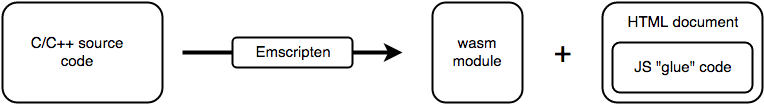
\includegraphics[height=1.75cm]{media/graphs/cpp_to_wasm.png}
        \captionsetup{justification=centering}
        \captionof{figure}{Od zdrojového kódu k .wasm modulu \cite{cpp_to_wasm_image}}
\end {center}

\subsection {Výsledná voľba prepojenia}
C\texttt{++} addons technológia je implementovaná v Node.js, čo by v prípade zvolenia tejto technológie znamenalo zvolenie architektúry klient-server.

Klientom by bol v tomto prípade webový prehliadač, ktorý by posielal HTTP požiadavku serveru s potrebnými dátami pre \texttt{grid-tracker} podprogram. Po skončení výpočtu by server poslal odpoveď s informáciami o bodoch a úsečkách, ktoré by mali byť vykreslené na všetkých importovaných snímkach magnetickej rezonancie.

V prípade použitia technológie WebAssembly by všetky výpočetné operácie mohli byť implementované na úrovni klienta. Tým pádom by nebolo nutné posielať žiadne dáta serveru, čo hrá v prospech bezpečnosti.

Avšak, ako z analýzy \texttt{grid-tracker} podprogramu vyplýva, \texttt{grid-tracker} a TNL knižnica pre zrýchlenie výpočetných algoritmov používajú OpenMP technológiu. Bohužiaľ, WebAssembly túto technológiu nepodporuje, čo by v tomto prípade znamenalo, že by celý výpočet musel prebiehať jednovláknovo alebo byť refaktorovaný tak, aby používal viacero vlákien pomocou technológie WebAssembly threads \cite{webassembly_threads} (vlastný preklad).

Čo sa týka C\texttt{++} addons, tá OpenMP technológiu podporuje. Taktiež by bol v rámci tejto technológie nutný menší zásah do zdrojového kódu \newline \texttt{grid-tracker} podprogramu, nakoľko by stačilo vytvoriť jednu wrapper funkciu v C\texttt{++}, ktorá by bola zodpovedná za konverziu dát do potrebného formátu a jeho výstup.

Taktiež nie je možné spoľahnúť sa na výkon zariadení, na ktorých by bežal \texttt{grid-tracker} pomocou WebAssembly. Nakoľko je tento algoritmus náročný na výpočet, bolo by potrebné zaistiť dostatočné výpočetné prostriedky pre každého lekára využívajúcim webovú aplikáciu.

Na základe týchto dôvodov bude lepšou a istejšou voľbou vybrať si technológiu C\texttt{++} addons, s ktorou by mala byť implementácia prepojenia \texttt{grid-tracker} podprogramu a webovej aplikácie jednoduchšia a s podporou OpenMP technológie. Výpočty v rámci \texttt{grid-tracker} podprogramu by taktiež neboli závislé na dostupných výpočetných prostriedkov klienta ale serveru, čo umožňuje mať väčšiu kontrolu nad potrebným škálovaním výkonu pre \texttt{grid-tracker} podprogram.

\clearpage

\section {Analýza frameworkov pre tvorbu webovej aplikácie}
Webovú aplikáciu je možné od základov naprogramovať len pomocou vlastného kódu, avšak takýto vývoj by bol nie len zdĺhavejší, ale aj pracnejší, nakoľko by sa musel samotný vývojár zamerať na viac než len na implementáciu samotnej aplikácie. Riešením je použitie webového frameworku, ktorý vývojára od takejto práce odbremenia. 

Pre vývoj webovej aplikácie by bolo vhodné využiť framework, ktorý je postavený nad Node.js technológiou, nakoľko by sa klientská a taktiež serverová časť aplikácie dala naprogramovať v jednom jazyku -- JavaScripte. Plusom by v tomto prípade bolo, ak by daný framework natívne podporoval TypeScript, čo by mohlo zredukovať prípadné chyby v implementácii webovej aplikácie.
Medzi ďalšími výhodami by patrilo použitie fullstack frameworku, vďaka ktorému by bolo potrebné orientovať sa len v jednom frameworku určenom pre obe časti webovej aplikácie -- frontend aj backend.

V súčasnosti medzi najviac používané fullstackové frameworky, ktoré \newline spĺňajú požiadavky uvedené vyššie, patria Nuxt.js\footnote{https://nuxt.com} a Next.js\footnote{https://nextjs.org}.

\subsection {Nuxt.js}
Nuxt.js je voľne dostupný open-source framework, pomocou ktorého je možné vytvárať fullstack webové aplikácie a stránky pomocou Vue.js\footnote{https://vuejs.org}. Vue.js technológia bude popísaná v samostatnej podsekcii nižšie.

Nuxt.js ponúka automatický routing na základe štruktúry súborov v \newline \texttt{/pages} zložke. Taktiež automaticky delí kód na menšie celky, čo môže pomôcť s prvým načítaním webovej aplikácie. Okrem renderovania obsahu až na klientovi je možné renderovať obsah už na serveri a takýto obsah poslať naspäť webovému prehliadaču. Pomocou automatických importov Vue.js komponentov nie je potrebné explicitne importovať použité Vue.js komponenty \cite{nuxt_introduction} (vlastný preklad).

Samotný framework je naprogramovaný v TypeScripte, čo znamená že je možné využívať type-hinty čo sa týka funkcionality Nuxt.js pri programovaní webovej aplikácie i bez nutnosti použitia TypeScriptu \cite{nuxt_introduction} (vlastný preklad).

Na pozadí používa Nuxt.js Nitro\footnote{https://nitro.unjs.io/} server, ktorý generuje API endpointy na základe štruktúry súborov nachádzajúcich sa v zložke \texttt{server/api} \cite{nuxt_introduction} (vlastný preklad).

Zostavenie aplikácie je možné pomocou príkazu \texttt{nuxt build} -- jeho výstupom je \texttt{.output} zložka obsahujúca minifikované súbory. Túto zložku je následne možné nasadiť na server podporujúci Node.js a zostavenú aplikáciu spustiť pomocou príkazu \texttt{node .output/server/index.mjs}.

\subsubsection {Vue.js}
Vue.js je JavaScript framework určený pre budovanie používateľského rozhrania postavený na štandardných technológiach ako HTML, CSS a JavaScript.

Tento framework poskytuje deklaratívny programovací model založený na znovupoužiteľných komponentoch, ktoré je možné použiť v rámci iných komponentov, čím pomáha zefektívniť proces vývoja znížením nutnosti použitia duplicitného kódu \cite{vuejs_introduction} (vlastný preklad).

Pod pojmom \uv{komponent} je možné predstaviť si samostatnú jednotku používateľského rozhrania (v HTML) s definovanými štýlmi (pomocou CSS) a stavom, ktorý je riadený pomocou JavaScriptu.
Takto definovaný komponent je možné nazvať tzv. Single File Componentom (SFC).

Nasleduje príklad využitia Vue.js frameworku -- pomocou vytvorenia SFC, ktorý v rámci jedného súboru kombinuje použitie HTML, CSS a JS ako v popise uvádzanom vyššie.

\clearpage
\begin{minipage}[]{\linewidth}
\begin{minted}{html}
// ParagraphComponent.vue
<template>
  <p>{{ paragraphText }}</p>
</template>

<script setup lang='ts'>
import { computed, defineProps } from 'vue';
const props = defineProps({
  text: {
    type: String,
    default: '',
  },
});
const paragraphText = computed(() => {
  return props.text;
});
</script>

<style lang='scss' scoped>
p {
  color: red;
}
</style>
\end{minted}
\end{minipage}

Uvedený príklad demonštruje dve hlavné funkcie Vue.js frameworku:
\begin {itemize}
\item {deklaratívne vykreslovanie a}
\item {reaktivitu \cite{vuejs_introduction} (vlastný preklad).}
\end {itemize}

V prvom prípade sa jedná o rozšírenie štandardného HTML o template syntax -- \{\{ \}\}, ktorý umožňuje dynamicky vykresliť obsah na základe JavaScript stavu.

V uvedenom príklade sa jedná o zobrazenie paragrafu, kde zobrazený text pochádza z premennej \texttt{paragraphText}. Táto premenná obsahuje \texttt{computed} funkciu, ktorá vracia hodnotu \texttt{props.text}.

Tá pochádza zo šablóny iného komponentu, kde bol tento komponent importovaný. Nasledujúci príklad zobrazuje šablónu tohto komponentu.

\clearpage

\begin{minipage}[]{\linewidth}
\begin{minted}{html}
// ArticleComponent.vue
<template>
  <paragraph-component text="Example text">
</template>

<script setup lang='ts'>
import { ParagraphComponent } from './ParagraphComponent.vue';
</script>
\end{minted}
\end{minipage}

V súbore \texttt{ArticleComponent.vue} bol importovaný komponent \newline \texttt{ParagraphComponent.vue}, ktorý definuje atribút \texttt{text} a nastavuje ho na hodnotu \uv{Example text}. Hodnota tejto premennej sa tým pádom spropaguje do
\texttt{ParagraphComponent.vue} komponentu do kľúča \texttt{text} objektu \texttt{props} (\texttt{props.text}).

\texttt{props} je objekt, v ktorom je možné nájsť všetky takto definované \texttt{properties}. Ak by sa namiesto fixného textu v atribúte \texttt{text} nachádzala premenná, ktorá by zmenila hodnotu, funkcia \texttt{computed} zaistí, že sa jej vrátená hodnota (\texttt{paragraphText}) zmení na základe detekovanej zmeny jej hodnoty.
Na základe tohto príkladu bola ukázaná sila reaktivity Vue.js frameworku.

Horeuvedeným spôsobom je možné modulárne vytvárať a zobrazovať rozličné komponenty podľa potreby. Taktiež je možné reagovať na rozličné eventy emitované prehliadačom, ako napr. na kliknutie myši na určitý element, posun po webovej stránke, atď.

Nakoľko webový prehliadač neumožňuje priamo importovať Vue.js komponenty, je nutné ich zostavením skonvertovať do JavaScriptu, napr. pomocou nástroja Vite\footnote{https://vitejs.dev} \cite{vuejs_introduction} (vlastný preklad).

Ten je nutné nainštalovať ako závislosť, napr. pomocou nástroja npm. Potom je potrebné vytvoriť konfiguračný súbor, v ktorom sa definuje zostavovanie Vue.js komponentov a následne pomocou príkazu \texttt{vite build} je možné zostaviť Vue.js komponenty do \texttt{.js} súborov, ktoré môžu byť následne importované do HTML šablóny \cite{vuejs_introduction} (vlastný preklad).

\clearpage

\subsection {Next.js}
Next.js je voľne dostupným, taktiež open-source fullstack frameworkom podobným Nuxt.js. Avšak narozdiel od Nuxt.js, Next.js nepoužíva pre vytváranie znovupoužiteľných UI komponentov knižnicu Vue.js ale React.js \footnote{https://react.dev/}.

Next.js ponúka nástroje pre vytváranie API endpointov, ktoré musia byť vytvorené v zložke \texttt{pages/api}. Čo sa týka samotnej funkcionality, taktiež podporuje kompilovanie UI komponentov do spustiteľného JS kódu, jeho minifikovanie pre rýchlejší prenos dát medzi serverom a webovým prehliadačom, code-splitting (rozdelenie kódu pre zvýšenie výkonu aplikácie) až po server-side rendering (SSR, vykreslený obsah na serveri sa pošle klientovi). Samotný framework je naprogramovaný pomocou TypeScriptu, takže je možné využívať nápovedu pri programovaní webovej aplikácie pomocou tohto frameworku \cite{nextjs_introduction} (vlastný preklad).

Zostavenie aplikácie je možné príkazom \texttt{next build}. Tento príkaz vytvorí \texttt{.next} zložku obsahujúcu skompilovaný obsah aplikácie. Takto skompilovanú aplikáciu je možné spustiť príkazom \texttt{next start} \cite{nextjs_introduction} (vlastný preklad). 

\subsubsection {React.js}
React.js je JavaScript framework, ktorý poskytuje možnosti pre budovanie používateľského rozhrania. Svojim účelom je podobný Vue.js frameworku a tiež patrí medzi open-source nástroj, ktorý je ale spravovaný spoločnosťou Meta\footnote{https://about.meta.com/} \cite{about_react} (vlastný preklad).

React.js sa od Vue.js líši spôsobom definovania komponentu -- nepoužíva SFC pre definovanie štruktúry komponentu, jeho štýlu a stavu ale tzv. JSX, ktorý umožňuje písať HTML v JavaScripte \cite{about_react} (vlastný preklad). \clearpage

JSX je oproti HTML striktnejší v tom, že:
\begin{itemize}
\item {samotný komponent musí byť uzatvorený v značke,}
\item {všetky značky musia mať uzatváraciu značku a}
\item {atribúty značiek je potrebné písať v camelCase forme \cite{jsx_rules} (vlastný preklad).}
\end{itemize}

Použitie CSS je v komponente možné pomocou importovania CSS stylesheetu napísaného pre daný komponent \cite{reactjs_stylesheet} (vlastný preklad), alebo importovania tzv. CSS modulu, ktorý je možné prepoužiť viacerými komponentmi \cite{reactjs_stylesheet_module} (vlastný preklad).

Taktiež je možné CSS definovať priamo v JS a ten naviazať priamo na element v komponente. CSS naviazané týmto spôsobom je možné dynamicky meniť v závislosti od vnútorného stavu komponentu.

Taémuto komponentu zostáva už len definovať jeho stav. Ten je možné vytvoriť pomocou funkcie \texttt{useState}, ktorého argumentom je inicializačná hodnota stavu. Táto funkcia vracia pole, kde na nultom indexe sa nachádza aktuálna hodnota daného stavu a na prvom indexe sa nachádza funkcia, ktorú je možné exekuovať pre aktualizáciu stavu \cite{react_state} (vlastný preklad).

Nasledujúci príklad zobrazuje použitie tejto funkcie:

\begin{minipage}[]{\linewidth}
\begin{minted}{typescript}
// ParagraphComponent.js
import { useState } from 'react';

const [answer, setAnswer] = useState('');
console.log(answer); // výstupom na konzole bude prázdny reťazec
setAnswer('foo');
console.log(answer); // výstupom na konzole bude reťazec 'foo'
\end{minted}
\end{minipage}

\clearpage

Pre porovnanie je na nasledujúcom príklade ukázaný rovnaký komponent ako v príklade pre Vue.js, avšak upravený pre React.js framework:

\begin{minipage}[]{\linewidth}
\begin{minted}{typescript}
import 'paragraph.css';

export default function Paragraph({ paragraphText = '' }) {
  return (
    <>
      <p> {paragraphText} </p>
    </>
  );
}
\end{minted}
\end{minipage}

V porovnaní s kódom pre Vue.js je horeuvedený kód kratší, nakoľko neobsahuje \uv{boilerplate} pre definovanie prijímaných properties ako vo Vue.js. Taktiež je automaticky zaistené prepojenie hodnoty \texttt{paragraphText} s vyrenderovaním jeho obsahu v \texttt{<p>} tagu. Pre fungovanie importovania horeuvedeného komponentu je potrebné funkciu, ktorá obsahuje definíciu React.js komponentu, exportovať. Táto povinnosť vo Vue.js odpadá.

Samozrejme je rozsah rozdielov väčší než tie uvedené v tejto práci. Účelom ukážky je informovať o základných rozdieloch vytvárania komponentov v oboch frameworkoch.

\subsection {Výsledná voľba frameworku}
Na základe doterajších skúseností s Vue.js frameworkom by mal byť vývoj aplikácie pomocou Nuxt.js frameworku pre autora plynulejší a menej problematický, keďže autor nemá skúsenosti s React.js a Nuxt.js frameworkom.

\clearpage

\section {Analýza spracovania MR snímiek}
Spracovávanie importovaných MR snímiek by malo čo v najväčšej miere prebiehať najmä na strane klienta -- vo webovom prehliadači. Takto zvolený prístup zamedzí prípadnému útočníkovi preniknúť k snímkam a dátam o pacientoch, ktoré by v opačnom prípade museli byť uchovávané na strane servera. Z uvedeného vyplýva, že pre implementáciu aplikácie bude potrebné nájsť JavaScript knižnicu resp. knižnice, ktoré sú schopné spracovať DICOM súbory v prehliadači.

Pod pojmom \uv{spracovať} je myslené: čítanie hlavičky DICOM súborov, zobrazenie snímiek nachádzajúcich sa v týchto súboroch, či možnosť tieto snímky modifikovať. Medzi ďalšie požiadavky kladené na takúto knižnicu patrí jej aktívny vývoj, dostupná dokumentácia a taktiež použiteľnosť knižnice pre produkčné nasadenie.

Bohužiaľ, všetky požiadavky kladené na hľadanú knižnicu nespĺňa ani jedna nájdená knižnica, ale výber viacero knižníc, kde každá z nich implementuje určitú časť požiadaviek a dokopy podmienky kladené na knižnicu vyššie, spĺňajú.

Jedná sa o nasledovné knižnice:
\begin {itemize}
\item {Cornerstone Core,}
\item {Cornerstone DICOM Image Loader a}
\item {Dicom Parser.}
\end {itemize}

\subsection {Cornerstone Core}
Cornerstone Core\footnote{https://github.com/cornerstonejs/cornerstone} je knižnica, ktorá má za úlohu zjednodušiť proces vývoja komplexnejších webových aplikácií, ktoré majú za úlohu zobrazovať snímky akéhokoľvek formátu, vrátane bežných medicínskych snímkových formátov. Taktiež poskytuje API, pomocou ktorého je možné zobrazovať DICOM snímky a samotné zobrazenie konfigurovať, ako napr. zvýšením alebo znížením intenzity jasi, priblížením a oddialením snímky, a iné \cite{about_cornerstone_core} (vlastný preklad).

Táto knižnica neimplementuje import DICOM súborov a ich spracovanie. Túto funkcionalitu deleguje na tzv. ImageLoaders. Tie po spracovaní DICOM súborov posunú DICOM dáta cez spoločné rozhranie Cornerstone Core knižnici, ktorá ich nakoniec vykreslí \cite{about_cornerstone_core} (vlastný preklad).

Cieľom tohto prístupu Cornerstone Core knižnice je jej dôraz na minimalizmus a poskytnutie flexibility pri spracovávaní rôznych typov obrazových dát. Použitie Cornerstone Core knižnice pre vývoj špecializovaných aplikácií tohto typu je de-facto štandardom \cite{about_cornerstone_core} (vlastný preklad).

V súčasnosti sa pripravuje nová \uv{Cornerstone Core} knižnica, ktorej názov sa zmení na \uv{Cornerstone3D}\footnote{https://github.com/cornerstonejs/cornerstone3D-beta}. Keďže je táto knižnica momentálne v beta berzii a stabilná verzia tejto knižnice ešte nebola vydaná, vývoj aplikácie bude postavený na doterajšej Cornerstone Core knižnici.
Momentálne neexistuje alternatíva tejto knižnice, ktorá by sa špecifikovala na túto oblasť.

\subsection {Cornerstone DICOM Image Loader}
Cornerstone DICOM Image Loader\footnote{https://github.com/cornerstonejs/cornerstone3D-beta/tree/main/packages/dicomImageLoader} je tzv. ImageLoader, ktorý je zodpovedný za načítanie a spracovanie DICOM súborov. Použitie tejto knižnice je vynútené Cornerstone Core knižnicou. Táto knižnica podporuje nielen načítanie DICOM súborov cez HTTP protokol, ale aj z lokálneho súborového systému pomocou File API\footnote{https://developer.mozilla.org/en-US/docs/Web/API/File\textunderscore API} implementovaného webovými prehliadačmi \cite{about_cornerstone_dicom_image_loader} (vlastný preklad).

Po načítaní DICOM súborov je ich parsovanie prenechané knižnici Dicom Parser. Nakoľko sa veľkosť týchto súborov môže pohybovať v rádoch megabajtov (MB), samotné parsovanie súborov prebieha pomocou využitia technológie Web Workers\footnote{https://developer.mozilla.org/en-US/docs/Web/API/Web\textunderscore Workers\textunderscore API}. Pre začiatok priblížim technológiu Web Workers a následne knižnicu Dicom Parser\footnote{https://github.com/cornerstonejs/dicomParser}.

\subsubsection {Web Workers}
JavaScript je v prehliadači implementovaný ako jednovláknový jazyk využívajúci jedno hlavné vlákno a exekúcia skriptov tohto jazyka prebieha zvyčajne v tomto vlákne. Výpočetne náročné úlohy by avšak mohli vyústiť do zablokovania tohto vlákna, ktoré sa prejavuje nereagovaním prehliadača na rozličné používateľské akcie alebo nevykreslovaním aktualizácií na webovej stránke. Dôvodom zablokovania hlavného vlákna by v tomto prípade bolo využitie všetkých dostupných prostriedkov prioritne pre danú výpočetne náročnú úlohu.

Web Workers technológia je štandardom, ktorý je implementovaný a poskytovaný webovými prehliadačmi umožňujúci exekúciu takýchto úloh, ktoré by inak pri dlhšom spracovávaní mohli dané hlavné vlákno zablokovať.

Pomocou Web Workers je možné predísť zablokovaniu hlavného vlákna jednoduchým vytvorením nového pracovného vlákna pomocou konštruktu \texttt{new Worker(url)}, kde \texttt{url} je adresa skriptu, ktorý má bežať v novom pracovnom vlákne. Takéto pracovné vlákno môže exekuovať JS skript bez zablokovania hlavného vlákna, keďže je od neho nezávislé a taktiež komunikovať s hlavným vláknom \cite{using_web_workers} (vlastný preklad).

\subsection {Dicom Parser}
Dicom Parser je knižnica implementujúca parsovanie všetkých známych validných DICOM súborov. Knižnica je navrhnutá pre beh vo všetkých moderných HTML5 prehliadačoch a nie je závislá na žiadnej knižnici \cite{about_dicom_parser} (vlastný preklad).

Dicom Parser poskytuje globálny objekt \texttt{dicomParser}, ktorý obsahuje viacero metód, z ktorých je najzaujímavejšia metóda \texttt{parseDicom}. Argumentom tejto metódy je \texttt{Uint8Array} pole obsahujúce nespracovaný (raw) obsah DICOM súboru. Výsledkom volania tejto metódy spolu s \texttt{Uint8Array} poľom je \texttt{DataSet} objekt obsahujúci vyparsovaný obsah DICOM súboru.

Alternatívou Dicom Parser knižnice by mohla byť knižnica dcm.js\footnote{https://github.com/dcmjs-org/dcmjs}, avšak vývoj tejto knižnice nie je stále dokončený (nebola zatiaľ vydaná jej stabilná verzia) a sami vývojári varujú pred použitím tejto knižnice v produkčnom prostredí\footnote{https://github.com/dcmjs-org/dcmjs}.

\subsection {Zhrnutie}
Pre zhrnutie informácií v tejto sekcii -- knižnica Cornerstone DICOM Image Loader využíva Web Workers pre vytvorenie nových pracovných vlákien, ktorých úloha je parsovanie DICOM súborov pomocou metódy \texttt{parseDicom} objektu \texttt{dicomParser} pochádzajúceho z Dicom Parser knižnice uvedenej vyššie. Metódou vrátený \texttt{DataSet} objekt je následne poslaný knižnici Cornerstone Core, ktorá sa postará o vykreslenie vyparsovanej DICOM snímky z tohto objektu.

\section {Analýza možností implementácie mriežky}
Pre implementáciu mriežky by bolo vhodné použiť knižnicu, pomocou ktorej by bolo možné danú mriežku vykresliť a upravovať podľa potrieb používateľa.

Rodina Cornerstone frameworkov ponúka pre tento účel knižnicu Cornerstone Tools\footnote{https://github.com/cornerstonejs/cornerstoneTools}, ktorá asistuje nielen pri vytváraní rôznych anotácií pre DICOM snímky (zobrazených pomocou Cornerstone Core), ale aj pri ich segmentácii či rôznych meraní. Taktiež ponúka široký počet nástrojov, ktoré môžu dané snímky modifikovať alebo nad týmito snímkami vykreslovať rôzne informácie či lomené čiary.

\subsection {Závislosti knižnice}
Pre využitie tejto knižnice je potrebná nielen Cornerstone Core knižnica, nakoľko je s ňou úzko previazaná, ale aj knižnica Hammer.js\footnote{https://github.com/hammerjs/hammer.js} a Cornerstone Math\footnote{https://github.com/cornerstonejs/cornerstoneMath}.

Cornerstone Tools využíva Cornerstone Core knižnicu pre reagovanie na rôzne eventy, ktoré Conerstone Core knižnica emituje. Na základe týchto eventov môžu nástroje Cornerstone Tools knižnice meniť svoj stav.

Hammer.js knižnica implementuje podporu rozhrania založeného na dotyku namiesto myši. Túto knižnicu je potrebné importovať bez ohľadu na to, či sa plánujú využívať gestá na báze dotyku alebo nie, nakoľko niektoré nástroje sú od tejto knižnice závislé.

Cornerstone Math, ako už názov napovedá, poskytuje rôzne matematické operácie týkajúce sa prevažne vektorovej matematiky. Niektoré nástroje z Cornerstone Tools knižnice ju používajú napr. pre výpočet vzdialenosti medzi rôznymi bodmi.

\subsection {Spôsoby implementácie mriežky}
Nakoľko Cornerstone Tools neobsahuje mriežku ako nástroj, ktorý vie knižnica zobraziť a s ňou ďalej pracovať, bude nutné ju od základov implementovať.

Táto implementácia môže využívať API\footnote{https://tools.cornerstonejs.org/api/} poskytované knižnicou, pomocou ktorej by bolo možné danú mriežku implementovať bez zásahu do knižnice alebo bude nutné danú mriežku naprogramovať priamo do knižnice.

\subsubsection {Implementácia pomocou Cornerstone Tools API}
Pri implementácii mriežky pomocou dedikovaného API by nebolo potrebné udržiavať vlastnú kópiu Cornerstone Tools knižnice. V tomto prípade by pre využitie rôznych funkcií implementovaných v samotnej knižnici bolo možné vyžadovanú funkcionalitu importovať pomocou metódy \texttt{importInternal(moduleName)}.

Nevýhodou tohto spôsobu je nedostatočná flexibilita spojená s nemožnosťou importovania všetkej funkcionality, ktorá by mohla byť pri vývoji potrebná. Ďalším negatívom zvolenia tohto spôsobu by bola nemožnosť upravenia akéhokoľvek kódu v Cornerstone Tools knižnici.

\subsubsection {Implementácia v rámci Cornerstone Tools knižnice}
Na druhú stranu, ak by mala byť mriežka implementovaná priamo v Cornerstone Tools knižnici, odpadol by problém s importovaním teoreticky potrebnej funkcionality, nakoľko by sa dal importovať akýkoľvek modul knižnice priamo pomocou JS konštruktu \texttt{import}, bez nutnosti využitia \texttt{importInternal} metódy.

\subsubsection {Výsledný výber spôsobu implementácie mriežky}
Nakoľko v tomto momente nie je jasné, či bude výsledná implementácia mriežky potrebovať zmenu niektorého zo súborov Cornerstone Tools knižnice, je vhodnejšie začať implementovať mriežku priamo v knižnici. Keď bude implementácia tejto mriežky dokončená, bude nutné posúdiť, či je možné celú funkcionalitu mriežky migrovať do riešenia využívajúceho iba dedikované API pre svoju funkcionalitu.

Ako pri Cornerstone Core, tak aj Cornerstone Tools knižnica bude mať čoskoro svojho nástupcu\footnote{https://github.com/cornerstonejs/cornerstone3D-beta/tree/main/packages/tools}, ktorá bude určená pre Cornerstone3D. Táto nová knižnica je momentálne v aktívnom vývoji a jej stabilná verzia rovnako ako v prípade Cornerstone3D nebola doteraz vydaná. To je dôvodom, prečo bude pri implementácii aplikácie použitá doterajšia verzia Cornerstone Tools knižnice.

\section {Zobrazenie závislostí medzi knižnicami}\label{dependency_graph}
Pre lepšie znázornenie previazania jednotlivých knižníc uvedených v tejto sekcii bol vytvorený diagram tried, na ktorom sú zobrazené instancie tried a závislosti medzi nimi.

\begin {center}
        \centering
        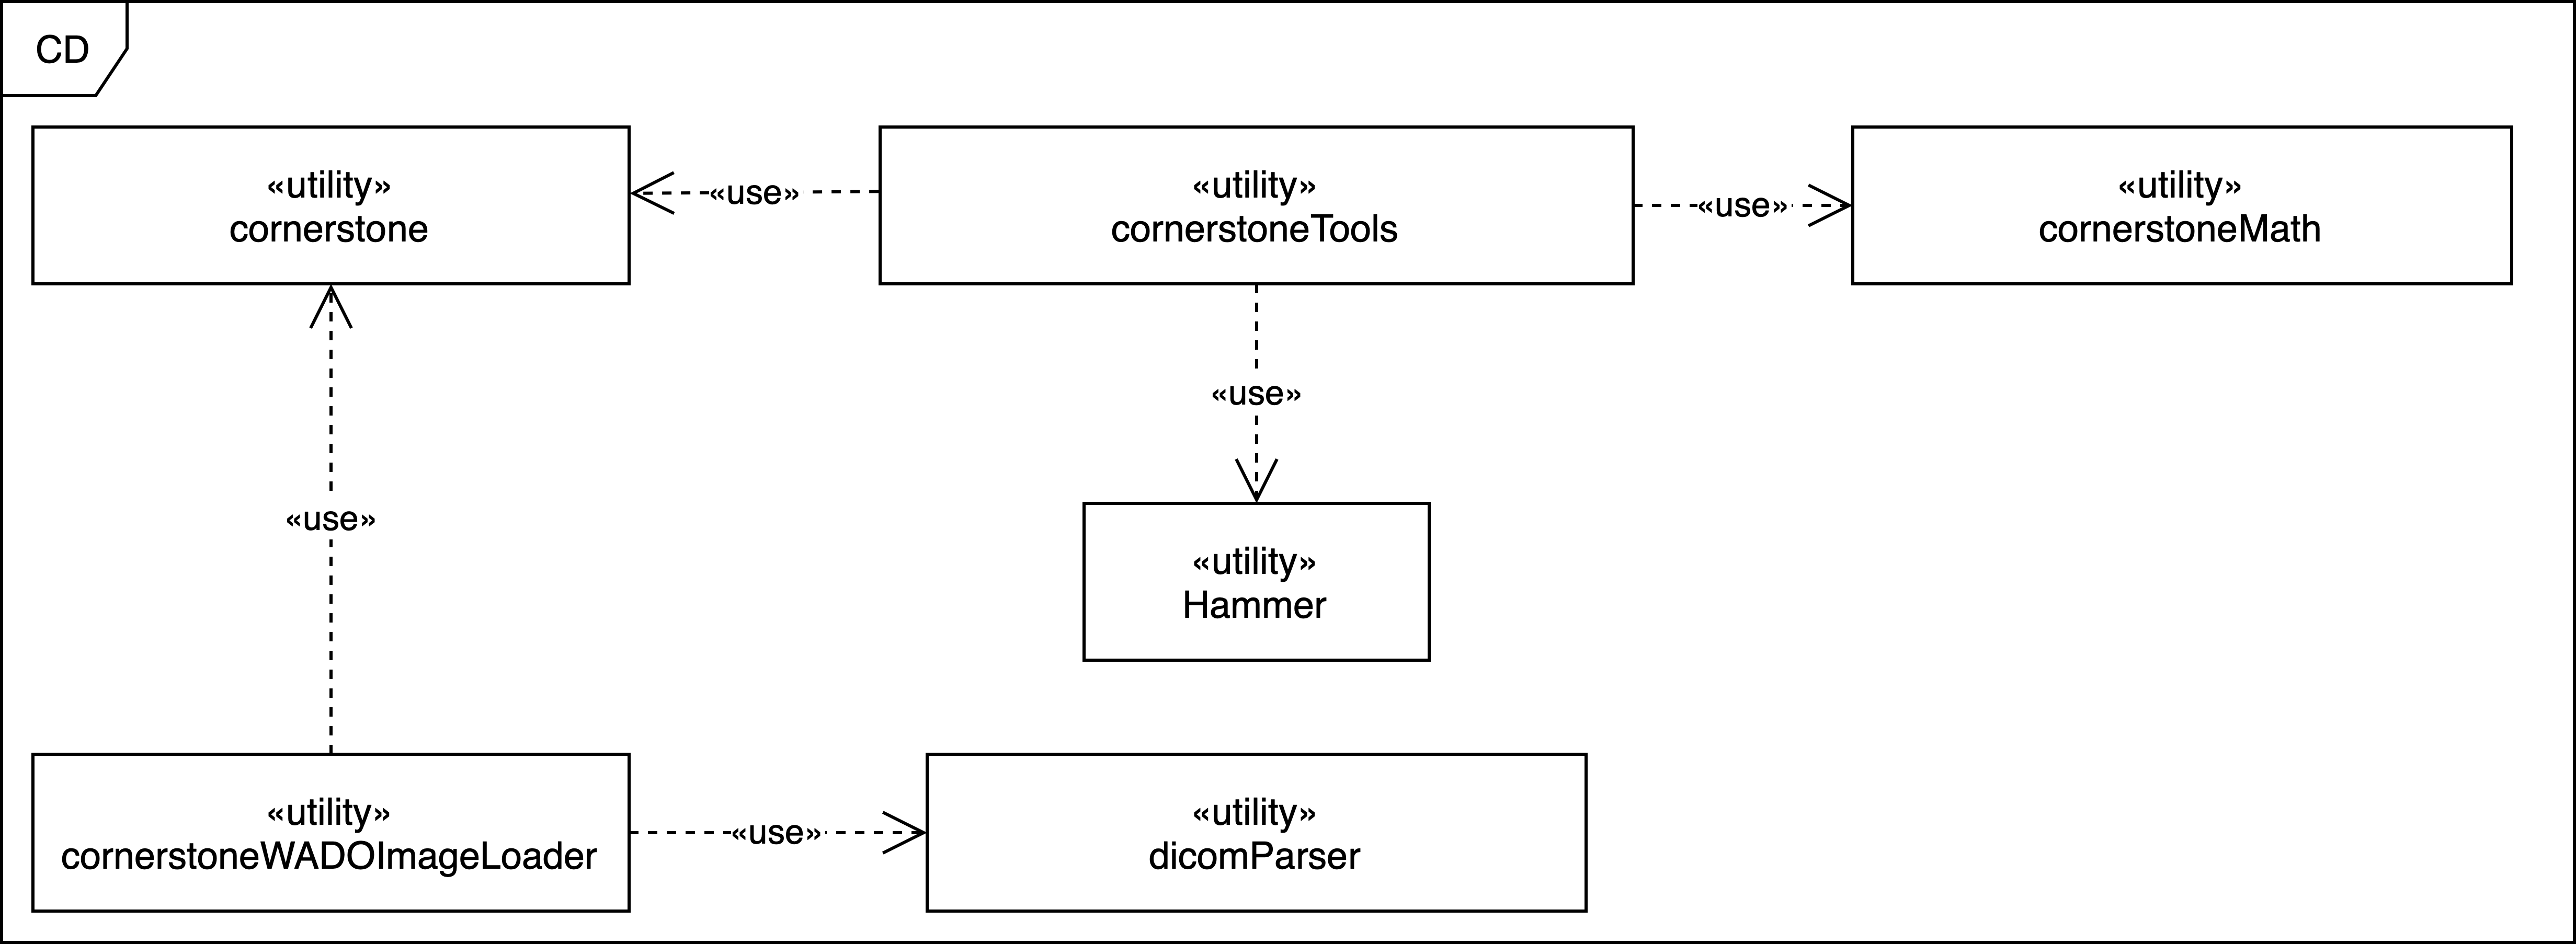
\includegraphics[height=4.75cm]{media/graphs/class_diagram.png}
        \captionsetup{justification=centering}
        \captionof{figure}{Class diagram znázorňujúci závislosti medzi knižnicami}
\end {center}

\clearpage

\section {Návrh používateľského rozhrania}
Pri návrhu používateľského rozhrania som sa inšpiroval UI doterajšej aplikácie, avšak s pár zmenami týkajúcimi sa štruktúry budúceho používateľského rozhrania.

Tento návrh používateľského rozhrania som rozdelil na 4 hlavné časti:
\begin {itemize}
\item {horný panel,}
\item {ľavý postranný panel,}
\item {centrálnu časť a}
\item {pravý postranný panel.}
\end {itemize}

Konečný návrh, ktorý bude slúžiť ako predloha pri vytváraní používateľského rozhrania webovej aplikácie, je priložený nižšie. Ten sa skladá z dvoch snímiek nakoľko sa obsah pravého postranného panelu môže meniť na základe zvolenej karty.

\begin {center}
\centering
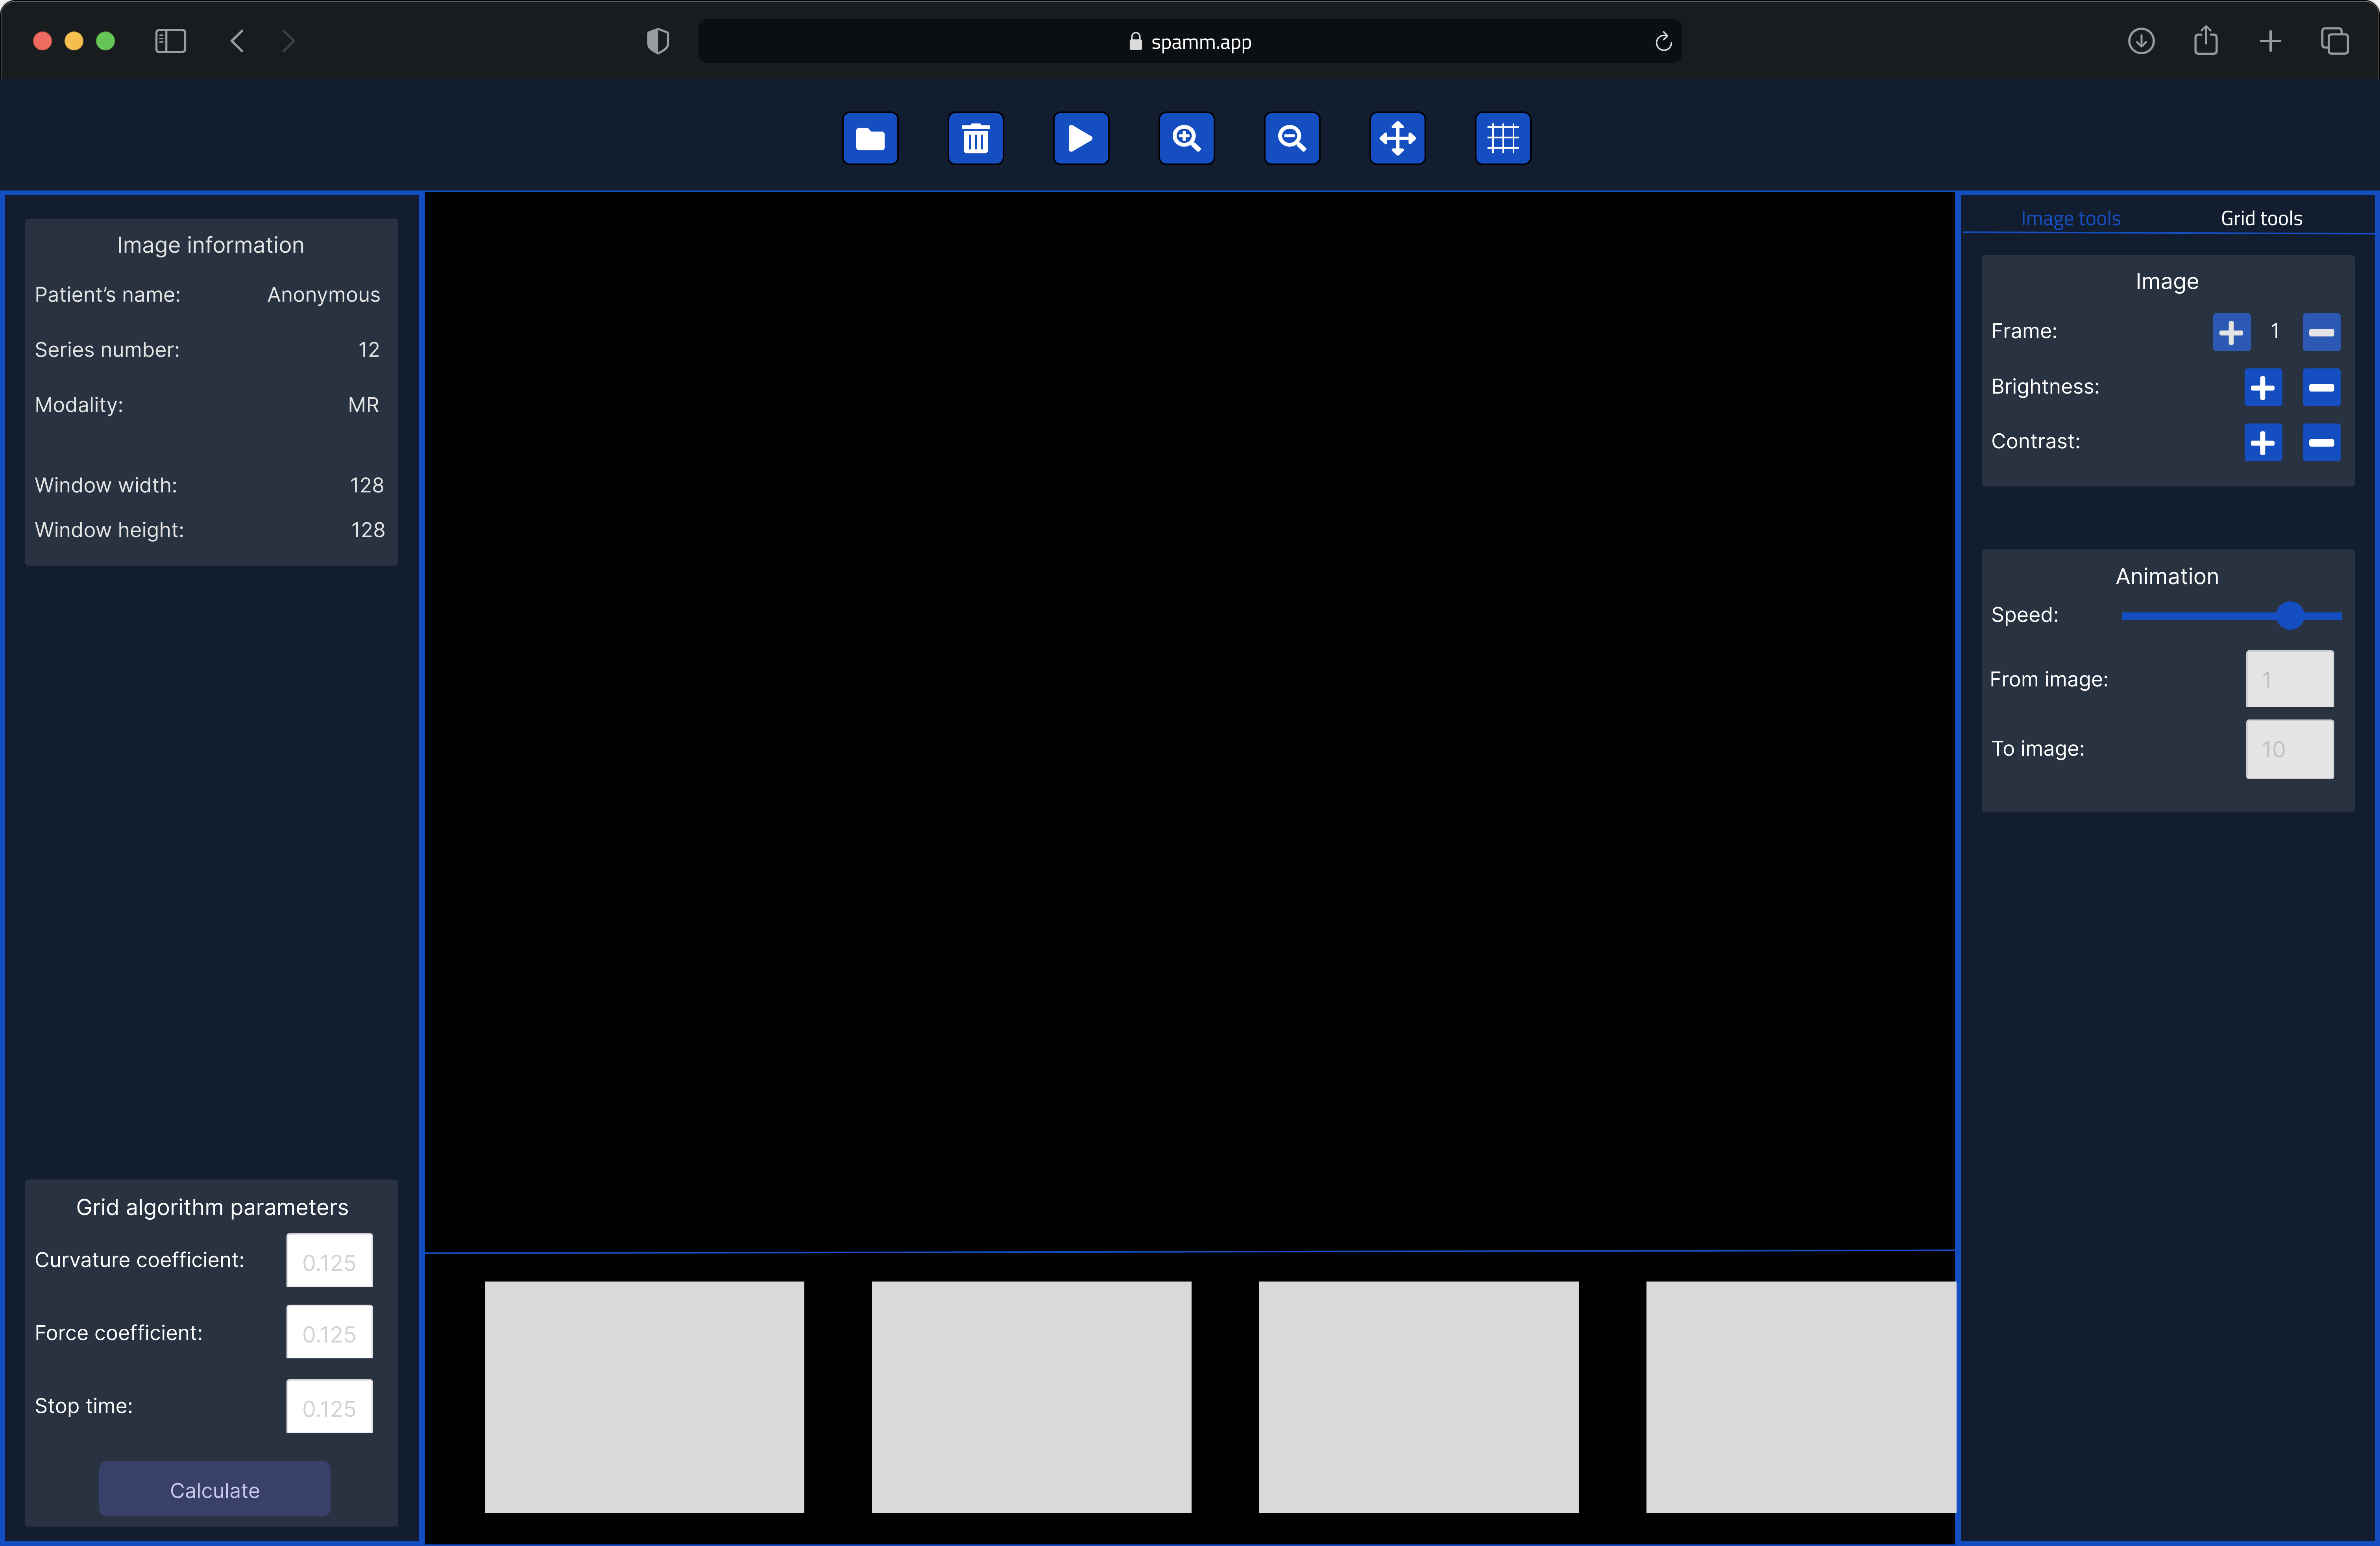
\includegraphics[height=8cm]{media/wireframes/1.png}
\captionsetup{justification=centering}
\captionof{figure}{Návrh používateľského rozhrania - prvá časť}
\end {center}

\begin {center}
\centering
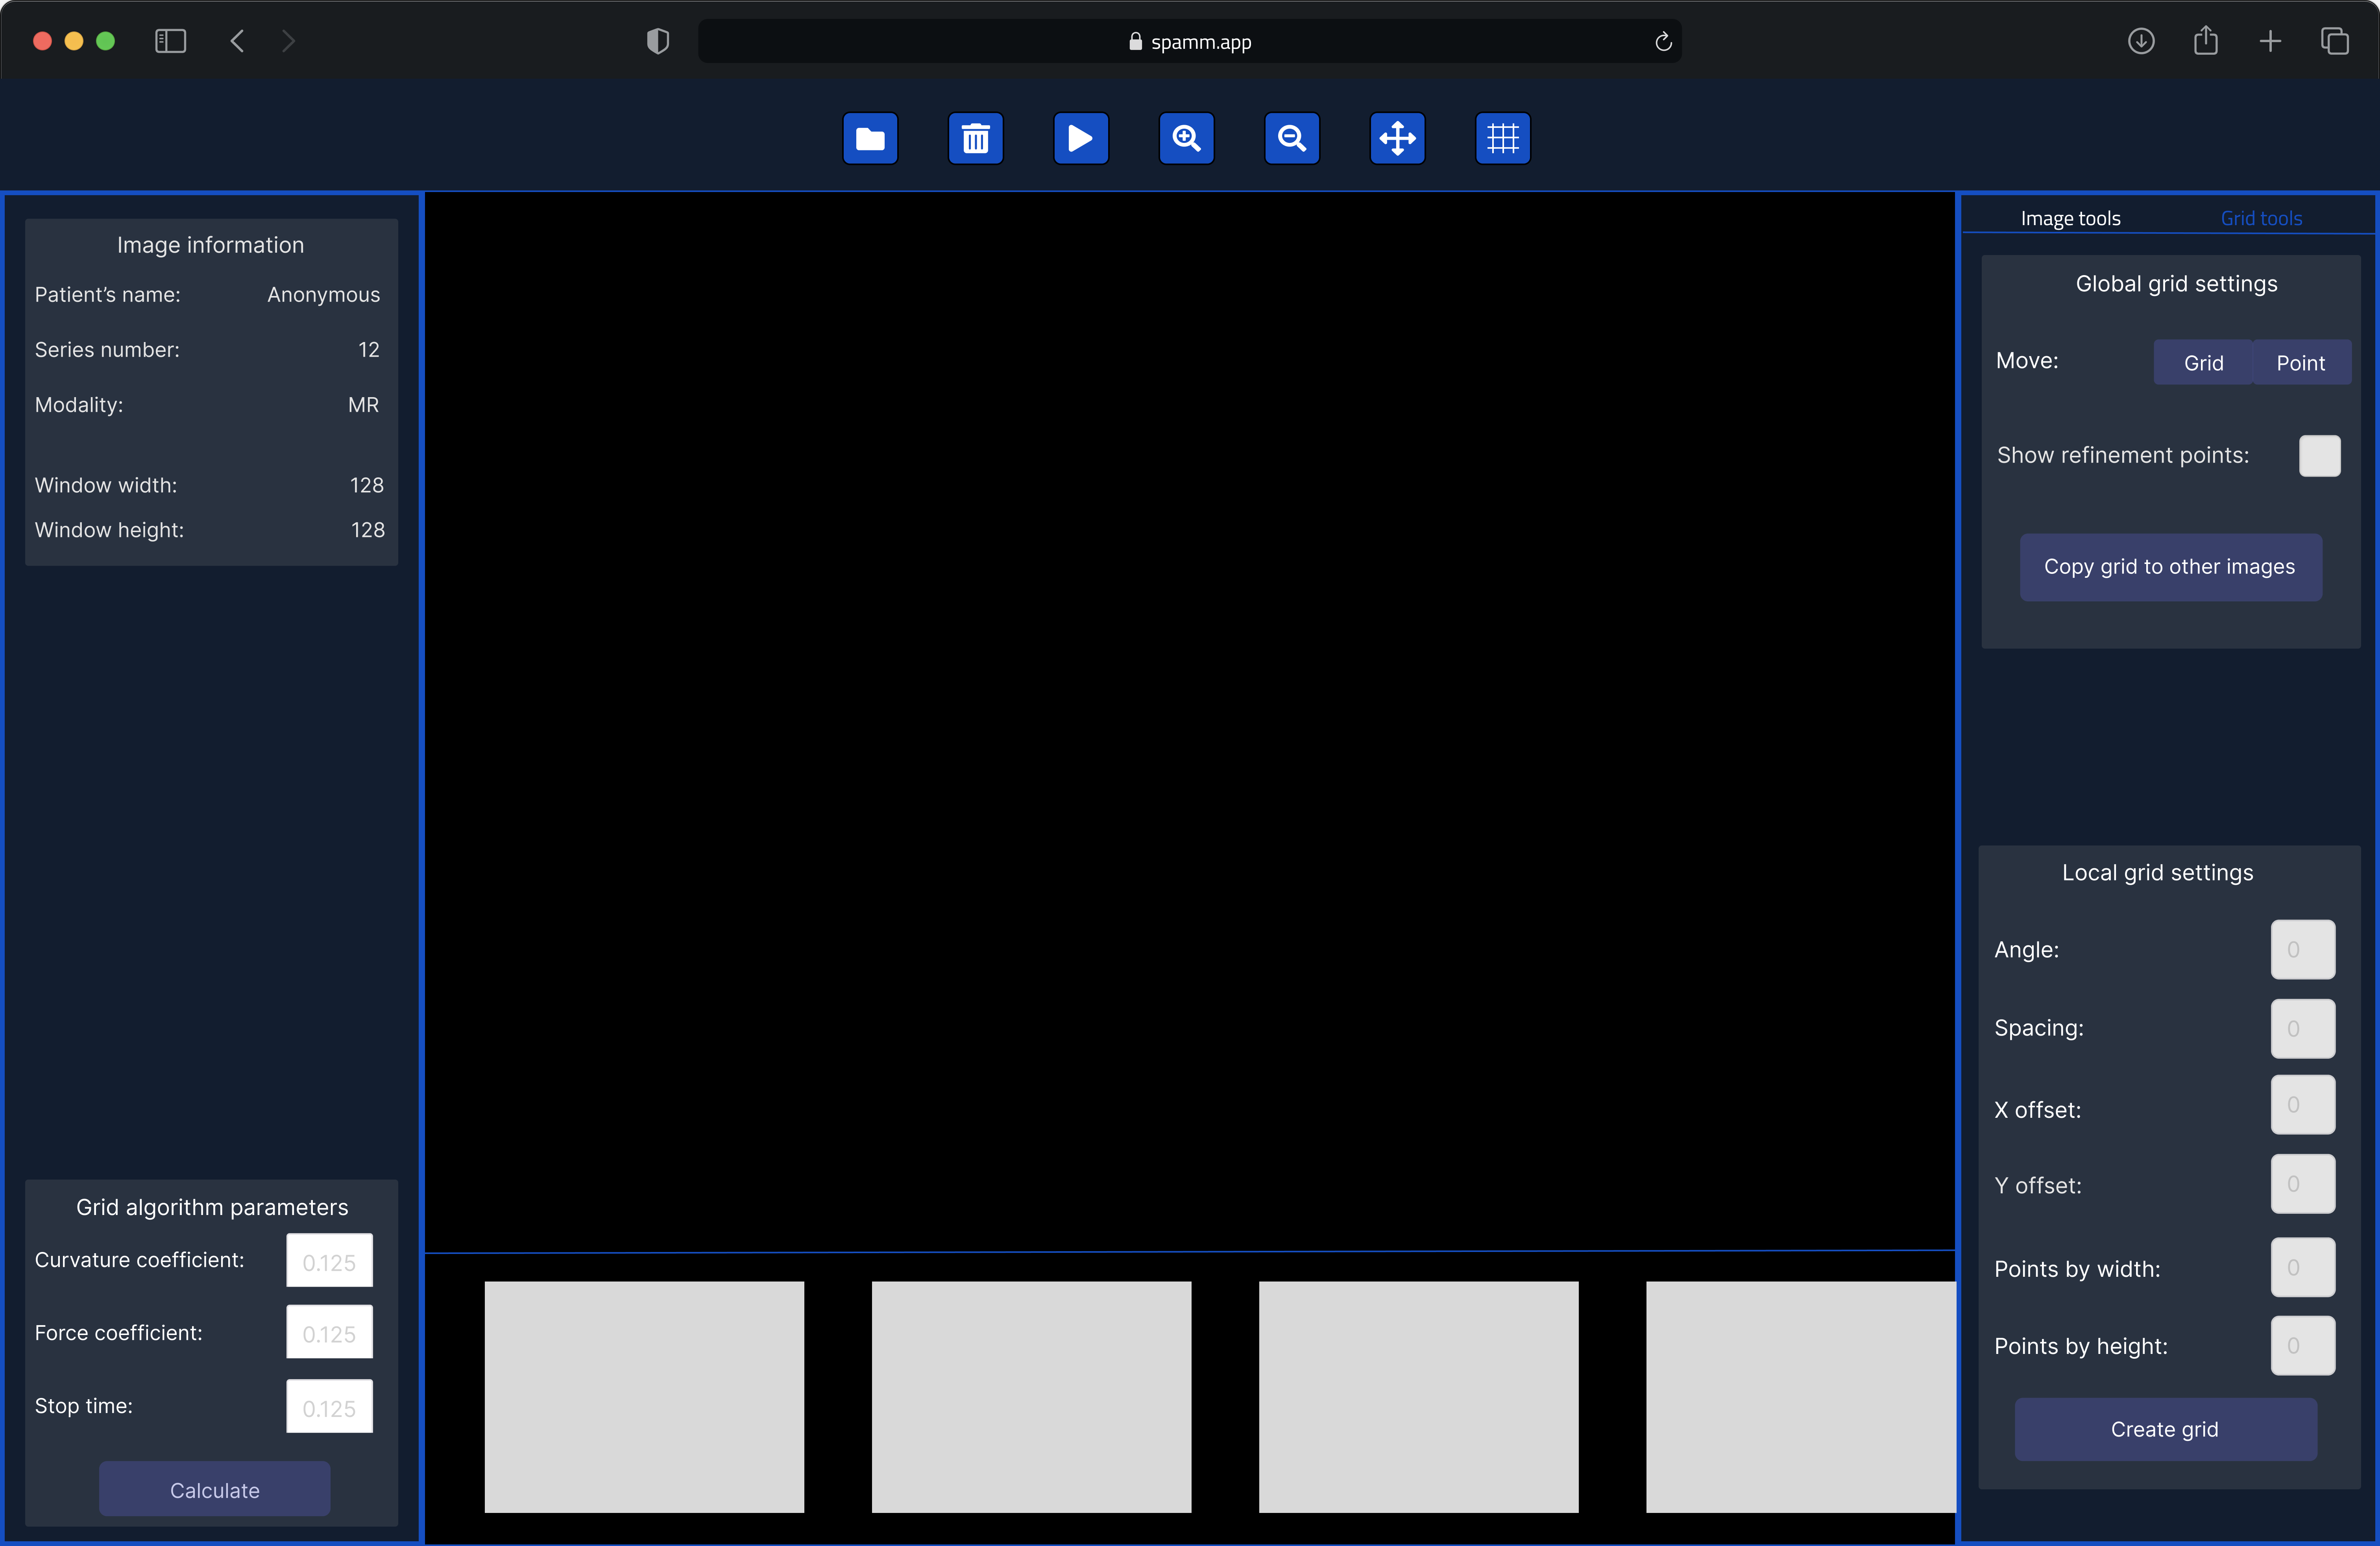
\includegraphics[height=8cm]{media/wireframes/2.png}
\captionsetup{justification=centering}
\captionof{figure}{Návrh používateľského rozhrania - druhá časť}
\end {center}

Nasledujúce podsekcie sa budú venovať popisu jednotlivých častí s popisom jednotlivých možností zobrazených v daných častiach.

\subsection {Horný panel}
V hornom paneli sa nachádzajú tlačidlá, na ktoré bude možné kliknúť.

Prvé tlačidlo zľava bude slúžiť pre načítanie DICOM snímiek. Po kliknutí naň sa zobrazí systémové okno, kde si používateľ bude môcť vybrať DICOM snímky, ktoré sa majú importovať do aplikácie. Pri každej tejto akcii sa vymažú doteraz importované snímky a nahradia sa práve importovanými snímkami.

Akonáhle používateľ aplikácie klikne na druhé tlačidlo, vymažú sa všetky načítané snímky a aplikácia sa prepne do stavu pred načítaním snímiek do aplikácie.

Tretie tlačidlo bude určené pre spustenie animácie snímiek. Po kliknutí naň sa ikona zmení na \uv{stop} ikonu a tlačidlo zmení svoju funkciu -- po opätovnom kliknutí sa animácia zastaví.

Pomocou štvrtého tlačidla bude možné priblížiť aktuálne zobrazenú DICOM snímku -- piate tlačidlo ju oddiali.

Šieste tlačidlo umožní posunúť DICOM snímku v ľubovoľnom smere a siedmym tlačidlom bude možné presúvať vykreslenú mriežku alebo jej body v závislosti na aktuálnom nastavení tohto tlačidla.

\subsection {Centrálna časť}
V centrálnej časti aplikácie bude zobrazená aktuálne vybraná DICOM snímka. Pod touto snímkou budú zobrazené náhľady na všetky importované snímky, ktoré bude možné zobraziť kliknutím na ne. Okrem zobrazenia samotnej snímky bude možné vykresliť používateľom definovanú mriežku, s ktorou bude možné interagovať pomocou myši.

\subsection {Ľavý postranný panel}
Ľavý postranný panel bude obsahovať dve sekcie -- \uv{Image information} a \uv{Grid algorithm parameters}.

\uv{Image information} sekcia bude informovať používateľa o mene pacienta nachádzajúceho sa na snímke. Okrem mena bude zobrazené číslo série a modalita, ktorej hodnota by pri skenoch MR mala byť rovnomenná (rovnajúca sa hodnote \uv{MR}). Pod týmito informáciami sa budú nachádzať informácie o výške a šírke zobrazenej snímky.

\uv{Grid algorithm parameters} bude slúžiť pre nastavenie parametrov SPAMM algoritmu. Tlačidlo \uv{Compute} bude predvolene vypnuté, dokým nebudú vytvorené mriežky na všetkých importovaných snímkach. V opačnom prípade bude možné kliknúť na toto tlačidlo, ktoré spracuje potrebné informácie z každej snímky a odošle požiadavku SPAMM algoritmu s potrebnými informáciami pre aktualizovanie súradníc bodov všetkých mriežok.

\clearpage

\subsection {Pravý postranný panel}
Pravý postranný panel bude rozdelený na dve karty -- \uv{Image tools} a \uv{Grid tools}. Pri kliknutí na jednu z možností sa obsah patriaci aktuálne zobrazenej možnosti skryje, aby bolo možné zobraziť obsah zvolenej karty.

\subsubsection {Image tools karta}
Na \uv{Image tools} karte bude možné zvoliť si snímku, ktorá sa má zobraziť. Okrem toho bude možné zmeniť jas a kontrast všetkých snímiek. Pod týmito nastaveniami bude možné upravovať nastavenia animácie snímiek, počínajúc nastavením rýchlosti animácie cez nastavenie počiatočnej a koncovej animovanej snímky.

\subsubsection {Grid tools karta}
\uv{Grid tools} karta bude obsahovať rozličné nastavenia mriežky. Tie sa rozdelia na globálne a lokálne nastavenia. Globálne nastavenia budú aplikované pre všetky vytvorené mriežky a lokálne nastavenia len na mriežku, ktorá je aktuálne zobrazená.

\subsubsection*{Globálne nastavenia mriežky}
V globálnych nastaveniach bude možné nastaviť možnosť interakcie s mriežkou pomocou myši (nastavenie \uv{Move}). Ak bude zapnutá možnosť \uv{Grid}, potiahnutím bodu mriežky sa celá mriežka posunie o vektor posunu. V prípade zvolenej možnosti \uv{Point} sa nebude posúvať celá mriežka, ale iba myšou zvolený bod mriežky.

Ďalšie nastavenie -- \uv{Show refinement points} -- bude slúžiť na dynamické pridanie, resp. odobranie \uv{refinement} bodov zo všetkých mriežok. Tzv. \uv{refinement} body slúžia pre presnejšie zarovnanie používateľom vygenerovanej mriežky so SPAMM mriežkou vygenerovanou MR prístrojom.

Po klliknutí na tlačidlo \uv{Copy grid to all images} sa zobrazí modálne okno, ktoré upozorní používateľa o možnosti skopírovania aktuálne zobrazenej mriežky do všetkých importovaných snímiek s možnosťou prípadného vrátenia tohto kroku. Toto tlačidlo bude aktívne iba v prípade, že na aktuálnej snímke bude zobrazená mriežka.

\subsubsection* {Lokálne nastavenia mriežky}
V lokálnych nastaveniach bude možné nastaviť rôzne parametre zobrazenej mriežky ako uhol, offset a iné. Pomocou tlačidla \uv{Create grid} bude možné vytvoriť mriežku s predvolenými nastaveniami. Po kliknutí naň sa tlačidlo zmení na \uv{Remove grid}, ktorého funkcia bude spočívať vo vymazaní mriežky na zobrazenej snímke.

\section {Návrh komunikácie webového rozhrania so serverom}\label{api_endpoint}
Pre potrebu komunikácie medzi serverom a klientom bude nutné túto komunikáciu navrhnúť. 

Serveru sa budú posielať dáta o používateľom definovaných mriežkach pre výpočet aktualizovaných súradníc bodov mriežok. Odpoveď klientovi by mala obsahovať aktualizované súradnice mriežok, ktoré webová aplikácia následne vykreslí.

V tomto prípade stačí, ak server bude poskytovať jeden REST API endpoint, ktorý potrebné dáta príjme, spracuje a odpoveď pošle klientovi vo dohodnutom formáte.

Detaily o tomto API endpointe sú nasledovné:
\begin {itemize}
\item {pre komunikáciu s endpointom bude využitý HTTP protokol,}
\item {endpoint bude dostupný na adrese \texttt{<hostname>/api/grid},}
\item {endpoint prijme dáta vtedy, ak daná požiadavka bude poslaná metódou POST a}
\item {telo požiadavky a odpovede budú vo formáte JSON.}
\end {itemize}

\clearpage

\subsection {HTTP požiadavka}\label{http_request}

Telo požiadavky bude mať nasledovný formát, ktorý je pre popis typov premenných popísaný v TypeScripte:

\begin{minipage}[]{\linewidth}
\begin{minted}{typescript}
{
  "data": [{
      "image": {
        "imageId": string;
        "imageData": Uint8Array;
      },
      "grid": {
        "includesRefinementPoints": boolean;
        "primaryLines": [{
            "points": [{
                "x": number;
                "y": number;
                "isCommonPoint": boolean;
              },
              ...
            ]
          },
          ...
        ]
      }
    }
  ]
}
\end{minted}
\end{minipage}

V \texttt{data} poli sa budú nachádzať objekty, z ktorých každý bude reprezentovať entitu skladajúcu sa zo štruktúry snímky (\texttt{image}) a jej mriežky (\texttt{grid}).

Hodnota \texttt{image} bude objektom, ktorého obsahom bude \texttt{imageId} reprezentujúci ID snímky a \texttt{imageData}, ktorý bude obsahovať pole binárnych dát DICOM súboru.

Hodnota \texttt{grid} bude taktiež objekt obsahujúci dva kľúče -- \texttt{primaryLines} a \newline \texttt{includesRefinementPoints}.

\texttt{primaryLines} bude reprezentovať pole zvislých úsečiek idúcich zľava doprava.
Obsahom každej takejto úsečky bude pole \texttt{points}, ktorého obsahom budú objekty reprezentujúce body na danej úsečke.

Každý bod sa bude skladať z troch kľúčov objektu: \texttt{x} -- reprezentujúci x-súradnicu bodu, \texttt{y} -- reprezentujúci invertovanú y-súradnicu bodu a príznak \texttt{isCommonPoint} značiaci, či je daný bod \uv{common} bodom (tzv. bod, v ktorom sa pretína vodorovná a zvislá úsečka mriežky) alebo \uv{refinement} bodom, pomocou ktorého je možné upresniť polohu mriežky. 

\texttt{includesRefinementPoints} značí, či sa v poli \texttt{points} nachádzajú aj tzv. \uv{refinement} body .

Používateľ iniciuje poslanie dát v tejto štruktúre kliknutím na tlačidlo \uv{Compute}.

\subsubsection {Anonymizácia DICOM dát}
Nakoľko obsahom požiadavky v rámci horeuvedeného API endpointu budú taktiež binárne dáta DICOM snímiek, bude nevyhnutné tieto snímky pred ich odoslaním na server anonymizovať takým spôsobom, aby nebolo možné spojiť snímky z magnetickej rezonancie s konkrétnym pacientom. Podľa \cite{Varma_2012} je nutné anonymizovať všetky DICOM tagy nachádzajúce sa v skupinách \uv{0008} a \uv{0010}. Skupina \uv{0008} obsahuje dáta ohľadom štúdie a skupina \uv{0010} obsahuje dáta o pacientovi.

Pre tento účel bude potrebné vytvoriť triedu reprezentujúcu DICOM anonymizér, ktorý bude implementovaný v JavaScripte na úrovni klienta. Táto trieda nahradí obsah tagov z horeuvedených skupín prázdnym reťazcom s dĺžkou daného tagu, aby nenastala inkonzistencia v DICOM dátach. Takto upravené dáta bude môcť byť bezpečne poslané na server.

\clearpage

\subsection{HTTP odpoveď}
Telo odpovede servera na požiadavku, ktorá bude obsahovať dáta o odoslaných mriežkach, bude v nasledujúcom formáte:

\begin{minipage}[]{\linewidth}
\begin{minted}{typescript}
{
  "grids": [{
    "imageId": string;
    "primaryLines": [{
      "points": [{
        "x": number;
        "y": number;
        "isCommonPoint": boolean;
      },
      ...
      ]
    },
    ...
    ]
  },
  ...
  ]
}
\end{minted}
\end{minipage}

Odpoveď bude obsahovať kľúč \texttt{grids}, ktorého obsahom budú objekty mriežok. Každý z týchto objektov bude obsahovať kľúč \texttt{imageId} a \texttt{primaryLines}.

Pomocou kľúča \texttt{imageId} bude možné spárovať objekt mriežky v odpovedi s mriežkou v aplikácii. Obsahom kľúča \texttt{primaryLines} bude pole zvislých úsečiek mriežky idúce zľava doprava.

Každá takáto úsečka bude obsahovať kľúč \texttt{points} reprezentujúci pole bodov v grafickej reprezentácii mriežky zhora nadol. Každý bod bude obsahovať svoje súradnice ($x$ a $y$) a príznak \texttt{isCommonPoint}, ktorý bude značiť, či je daný bod bodom, v ktorom sa pretína vodorovná a zvislá úsečka mriežky (\uv{common} bod) alebo nie (\uv{refinement} bod).